% 2026 全国规范电子版唯一正式入口。
% 不要移除 withoutpreface 或 notoc：电子版不得包含承诺书、编号页或目录。
% 使用 TeX Live 自带的 Fandol 中文字体，避免依赖本机 STSong/STHeiti。
\PassOptionsToPackage{fontset=fandol}{ctex}
\documentclass[withoutpreface,notoc,bwprint]{cumcmthesis}

% 公共宏包、图片路径与自定义命令。
% 使用 Sustainable-Enjoyment 模板本身的视觉样式。
% 旧样式已归档至 archive/legacy-template-files/cumcm2026.sty，不再加载，
% 避免覆盖上游标题、间距与图表样式。
\usepackage[super,numbers,sort&compress]{natbib}
% Noto Sans Mono 覆盖代码中的摄氏度等符号；中文仍由 ctex 字体回退处理。
\newfontfamily\CumcmCodeFont{NotoSansMono-Regular.ttf}
\newcolumntype{C}{>{\centering\arraybackslash}X}
\newcolumntype{R}{>{\raggedleft\arraybackslash}X}
\newcolumntype{L}{>{\raggedright\arraybackslash}X}
\BeforeBeginEnvironment{tabular}{\zihao{-5}}
% 给上游代码行号和外框留出内侧空间，防止侵入25mm页边距。
\lstset{basicstyle=\CumcmCodeFont\small,xleftmargin=12pt,xrightmargin=4pt}
\pagestyle{plain}
\hypersetup{pdfauthor={},pdfsubject={CUMCM 2026}}
\newcommand{\CumcmAIUsed}[1]{\section*{AI工具使用声明}本参赛队在竞赛过程中使用了AI工具，主要用于#1，详细使用情况见支撑材料中的《AI工具使用详情.pdf》。}
\newcommand{\CumcmAINotUsed}{\section*{AI工具使用声明}本参赛队在竞赛过程中未使用任何AI工具。}

% 正式图片优先，其次是可编辑图源和上游模板示例图片。
\graphicspath{{figures/final/}{figures/source/}{figures/}}

% 常用数学记号可在此集中定义，避免各章节重复声明。
\newcommand{\dif}{\mathop{}\!\mathrm{d}}


% 论文标题等基本信息。
% 电子版仅显示论文题目，不填写作者、学校、赛区或队号。
\title{热风烘干过程中药材径向传热传质与收缩耦合建模}


\begin{document}

\maketitle
% 上游首页隐藏页码；2026 规范要求摘要页从 1 开始编号。
\thispagestyle{plain}

% 摘要页。
\begin{abstract}
热风烘干过程中，药材表面首先受到环境作用，而内部温度和水分浓度以不同时间尺度向中心响应；当药材发生收缩时，传递距离和有效物性又会同步变化。为回答预热状态、全过程演化、全域达标时间及收缩影响四个递进问题，本文将药材理想化为轴对称长圆柱，构建统一的径向传热传质模型，并在结果层面区分局部状态、全域判停和移动表面三类输出。

针对问题一，采用附录2物性和固定半径的一维 Fourier 导热—Fick 扩散解耦模型，将附件1环境序列分段线性插值为连续边界；针对问题二，在相同几何下引入附录3的含水率相关密度、比热容、导热系数及温度—含水率相关扩散系数，形成同步更新的热质参数耦合模型；针对问题三，沿用问题二的全过程描述，以轴线、内部控制体和真实表面水分浓度的最大值定义连续终止事件；针对问题四，依据附件2半径轨迹和附录4物性，在材料坐标 $\xi=r/R(t)$ 下处理径向收缩，并对固定物理位置出域和实时表面分别输出。

空间上采用守恒有限体积法，内部界面物性取调和平均，表面状态由半网格关系重构；时间上采用 BDF 方法同步推进温度和水分。问题一计算表明，$1800\,\mathrm{s}$ 时中心与表面温度分别为 $33.5753$ 和 $36.7856\,{}^\circ\mathrm{C}$，对应水分浓度分别为 $2.5500$ 和 $1.5102\,\mathrm{kg/kg}$，热响应已进入内部而失水仍集中在表层。问题二的前三小时结果显示，温度场先于水分场趋于均匀，至 $3\,\mathrm{h}$ 轴线与表面温度分别为 $49.8495$ 和 $49.9664\,{}^\circ\mathrm{C}$，而水分浓度仍为 $1.7662$ 和 $1.0081\,\mathrm{kg/kg}$，内部传质滞后明显。

在固定半径、附录3物性条件下，问题三得到全域水分浓度首次达到 $0.15\,\mathrm{kg/kg}$ 的时间为 $57.17\,\mathrm{h}$。考虑附录4物性和附件2径向收缩后，问题四的连续临界时刻为 $182956.15\,\mathrm{s}$（约 $50.82\,\mathrm{h}$）；终点半径为 $1.2000\,\mathrm{cm}$，全域最大值位于轴线，表面水分浓度约为 $0.0525\,\mathrm{kg/kg}$。四工况对照表明，物性变化和几何收缩共同决定达标时间，不能将问题三与问题四的时间差全部归因于收缩。

网格加密、时间积分设置、全域守恒、跨问题对齐、零扩散极限、固定域退化复现及代表时刻边界根扫描共同支持给定假设下的数值可靠性与模型内部一致性。模型主要适用于圆柱主体的径向过程；长度不变、材料同比例收缩、环境数据末值延拓以及未显式加入蒸发潜热等处理，限定了结果向实际工艺推广时的适用范围。

\keywords{热风烘干\,径向传热传质\,变物性耦合\;移动边界\,全域达标判定}
\end{abstract}


% 正文。按文件拆分，方便并行写作和版本管理。
\section{问题重述}

\subsection{问题背景}

热风烘干通过调节烘房的温湿环境，使中药材经历预热平衡与恒温干燥两个阶段。
工艺参数的选择关系到干燥效率、能耗及成品品质，而依靠反复试验优化工艺需要较高的时间与成本投入。
因此，需要借助数学模型描述药材内部温度与水分浓度的时空变化，并据此确定满足烘干要求的处理时间。

题目所给药材近似呈圆柱形，初始长度为 $25\,\mathrm{cm}$、半径为 $2\,\mathrm{cm}$，
初始温度为 $28\,{}^\circ\mathrm{C}$，初始水分浓度为 $2.55\,\mathrm{kg/kg}$。
其中，药材的水分浓度指干基含水率。
附件1给出烘干初期烘房温度和水分浓度随时间的变化，附件2给出烘干过程中药材半径的变化，
题面附录2至附录4分别提供各问题所需的物性参数或经验公式。
在这些条件下，需要依次研究阶段内变化、全程变化、达标时间及尺寸收缩的影响。

\subsection{具体问题}

\textbf{问题一：预热平衡阶段的温度与水分浓度变化。}
根据附件1的烘房环境数据及题面附录2的参数，建立预热平衡阶段的数学模型，
求出前 $1800\,\mathrm{s}$ 内药材温度与水分浓度的时空分布。
在 $100$、$300$、$600$、$900$、$1200$、$1500$ 和 $1800\,\mathrm{s}$，
给出距药材中心 $0$、$0.5$、$1$、$1.5$ 和 $2\,\mathrm{cm}$ 处的两类结果。

\textbf{问题二：整个烘干过程的温度与水分浓度变化。}
将研究范围由预热平衡阶段扩展至包含恒温干燥阶段的全过程，
统一采用题面附录3的经验公式，描述密度、比热容、热传导系数随含水率的变化，
以及水分扩散系数对含水率和温度的依赖。
建立相应模型，并给出前 $3\,\mathrm{h}$ 内每隔 $0.5\,\mathrm{h}$、上述五个位置的温度与水分浓度。

\textbf{问题三：满足含水率要求的烘干时间。}
沿用问题二的全过程描述和题面附录3的经验公式，
以药材各处水分浓度均低于 $0.15\,\mathrm{kg/kg}$ 为结束条件，确定所需烘干时长，以小时计。
给出烘干过程中每隔 $6\,\mathrm{h}$ 及烘干结束时、距中心每隔 $0.5\,\mathrm{cm}$ 处的水分浓度。

\textbf{问题四：考虑尺寸收缩的烘干时间。}
在问题三的达标要求下，进一步考虑水分流失引起的药材尺寸变化，
依据附件2的半径数据及题面附录4的经验公式，确定药材收缩时的烘干时长。
给出每隔 $6\,\mathrm{h}$ 及烘干结束时的水分浓度，位置按距中心 $0.5\,\mathrm{cm}$ 的间隔选取，
并包含各时刻的药材表面。

题目要求的正文结果表及结果工作簿中的温度、含水率场值统一保留四位小数；连续事件时刻及数值检验指标按分析需要保留必要有效位数。正文结果按题面表1至表6的格式列示。
完整结果按附件3提供的 \texttt{result1.xlsx} 至 \texttt{result4.xlsx} 模板保存。
其中，问题一、二的完整结果采用 $1\,\mathrm{s}$ 的时间间隔，问题三、四采用 $60\,\mathrm{s}$ 的时间间隔，
空间间隔均为 $0.1\,\mathrm{cm}$。

\section{问题分析}

\subsection{问题一的分析}
问题一研究前 $1800\,\mathrm{s}$ 的预热阶段。附件1给出离散环境数据，题面要求输出指定时刻和径向位置的温度与水分浓度。因此，本问的核心是将环境序列转化为连续边界，在固定半径的一维径向圆柱模型中分别求解导热和水分扩散过程，并以守恒离散保证表面通量与内部变化相容。

\subsection{问题二的分析}
问题二将时间范围扩展至前三小时，并采用附录3的变物性关系。相较问题一，密度、比热容和导热系数随含水率变化，水分扩散系数同时依赖含水率和温度，温度场与水分场由此形成参数耦合。本问仍采用固定半径和相同环境边界，重点分析温度快速响应与水分扩散滞后的差异。

\subsection{问题三的分析}
问题三要求确定全域水分浓度达到阈值的时间。它继承问题二的固定域耦合模型，仅增加长时段积分和全域事件判定。判停量取轴线、控制体及真实表面水分浓度的最大值，避免以表面或单一采样点代替整个药材的达标条件；附件1结束后的环境量按末值延拓，并对该边界假设进行敏感性分析。

\subsection{问题四的分析}
问题四同时改变几何和物性条件。附件2给出半径随时间的变化，附录4给出新的经验物性；固定物理位置还可能随收缩移出药材域。本问用材料坐标 $\xi=r/R(t)$ 将移动区域映射到固定区间，使收缩体现为传递尺度 $R(t)^{-2}$，并在输出时区分固定位置和实时表面。除比较最终临界时间外，还需检验移动模型在固定域和零扩散极限下的自洽性。

\subsection{统一求解与结果组织}
四问采用统一的轴对称径向传递框架和守恒有限体积离散；问题二至四同步更新状态相关物性，问题三、四以全域最大水分浓度触发连续事件。结果章节按“模型的建立—模型的求解—结果的得出与分析”组织，数值可靠性和敏感性在统一章节中汇总。

\begin{table}[H]
\centering
\caption{四个问题的建模递进与主要输出}
\label{tab:problem-analysis}
\zihao{-5}
\begin{tabular}{@{}lccc@{}}
\toprule
问题 & 几何与物性 & 主要计算量 & 主要输出 \\
\midrule
一 & 固定半径、附录2 & 解耦温度与水分场 & 指定时刻和位置场值 \\
二 & 固定半径、附录3 & 变物性耦合场 & 前三小时场值 \\
三 & 固定半径、附录3 & 全域事件积分 & 达标时间与径向分布 \\
四 & 径向收缩、附录4 & 移动域耦合场 & 达标时间、表面及影响对照 \\
\bottomrule
\end{tabular}
\end{table}

\section{模型假设}

\begin{enumerate}
\item 药材近似为均匀、各向同性的长圆柱，长度 $L=0.25\,\mathrm{m}$；模型只描述径向传热传质，忽略周向和轴向变化，主要适用于圆柱主体区域。
\item 问题一至三半径保持不变；问题四长度不变，仅发生径向收缩，材料位置随半径同比例缩放，并用材料坐标描述几何运动。
\item 初始温度和干基水分浓度在药材内部均匀分布，温度采用 Fourier 导热方程，水分采用 Fick 扩散方程；表面采用第三类对流边界，轴线采用轴对称零通量条件。
\item 附件1环境数据在给定时间范围内分段线性插值；长时段计算超出数据范围时，环境量保持为附件末值。问题四的半径轨迹由附件2数据插值确定。
\item 本文不显式考虑蒸发潜热、吸附等温线、Soret/Dufour 效应及未经题面给出的收缩本构关系。这些是模型简化，不表示相应机制在实际过程中不存在。
\end{enumerate}

上述假设限定了模型的适用范围；网格、时间积分和表面重构属于数值实现，在各问题的求解与检验部分说明。

\section{符号说明}

% 符号定义维护于 docs/notations.md；增补或改名时同步更新两处。
% 使用 longtable 保留续表表头，后续新增条目无需压缩字号或行距。
本文主要符号及单位见表\ref{tab:notations}。
下标 $a$、$s$、$0$ 分别表示烘房空气、药材表面和初始状态，
正文中的 $T$、$T_a$ 和 $T_s$ 统一采用摄氏温度，单位为 ${}^\circ\mathrm{C}$。凡进入 Arrhenius 经验公式，单独定义 $T_K=T+273.15$，并以 $T_K$ 代入指数项；后续各问均遵循此约定。

\begingroup
% 与项目 tabular 表格沿用相同字号、行距，不修改公共模板。
\zihao{-5}
\renewcommand{\arraystretch}{1.38}
\begin{longtable}{@{}p{0.13\textwidth}p{0.60\textwidth}p{0.20\textwidth}@{}}
\caption{核心符号及单位}\label{tab:notations}\\
\toprule
符号 & 含义 & 单位 \\
\midrule
\endfirsthead
\multicolumn{3}{c}{\textbf{表\thetable\quad 核心符号及单位（续）}}\\
\toprule
符号 & 含义 & 单位 \\
\midrule
\endhead
\midrule
\multicolumn{3}{r}{续下页}\\
\endfoot
\bottomrule
\endlastfoot
$t$ & 烘干时间 & $\mathrm{s}$ \\
$t_e$ & 全域最大水分浓度首次降至阈值的临界时刻 & $\mathrm{s}$ \\
$\xi$ & 材料坐标，$\xi=r/R(t)$ & $1$ \\
$C_{\max}$ & 全域最大水分浓度 & $\mathrm{kg/kg}$ \\
$r$ & 到圆柱中心轴的径向距离 & $\mathrm{m}$ \\
$R$ & 药材半径；尺寸变化时记为 $R(t)$ & $\mathrm{m}$ \\
$L$ & 药材长度 & $\mathrm{m}$ \\
$T$ & 药材温度，正文采用摄氏温度 & ${}^\circ\mathrm{C}$ \\
$C$ & 药材水分浓度，即干基含水率 & $\mathrm{kg/kg}$ \\
$\rho$ & 药材密度 & $\mathrm{kg/m^3}$ \\
$c_p$ & 药材比热容 & $\mathrm{J/(kg\cdot K)}$ \\
$k$ & 热传导系数 & $\mathrm{W/(m\cdot K)}$ \\
$D$ & 水分扩散系数 & $\mathrm{m^2/s}$ \\
$h$ & 对流换热系数 & $\mathrm{W/(m^2\cdot K)}$ \\
$h_m$ & 对流传质系数 & $\mathrm{m/s}$ \\
$T_a$ & 烘房空气温度，正文采用摄氏温度 & ${}^\circ\mathrm{C}$ \\
$C_a$ & 烘房空气水分浓度，采用附件口径 & $\mathrm{kg/kg}$ \\
$T_s$ & 药材表面温度，正文采用摄氏温度 & ${}^\circ\mathrm{C}$ \\
$C_s$ & 药材表面水分浓度，即表面干基含水率 & $\mathrm{kg/kg}$ \\
$\alpha$ & 热扩散率，$\alpha=k/(\rho c_p)$ & $\mathrm{m^2/s}$ \\
$\tau_T$ & 径向热扩散特征时间 & $\mathrm{s}$ \\
$\tau_C$ & 径向水分扩散特征时间 & $\mathrm{s}$ \\
$N$ & 径向控制体总数 & $1$ \\
$\Delta r$ & 均匀径向网格宽度 & $\mathrm{m}$ \\
$i$ & 控制体或节点编号 & $1$ \\
\end{longtable}
\endgroup

表中单位“$1$”表示无量纲。
物性参数及数值离散符号均在相应问题中定义。

\section{问题一：预热平衡阶段的温度与水分浓度}

问题一要求根据附件1给出的烘房环境变化，求出预热平衡阶段药材内部温度和水分浓度的时空分布，并在指定时刻和径向位置给出结果。该阶段的主要困难在于：热量和水分均从圆柱表面传入或传出，内部响应具有明显的径向梯度；同时，附件1只给出离散环境数据，不能直接作为连续时间边界条件使用。

药材长度为 $L=0.25\,\mathrm{m}$，半径为 $R=0.02\,\mathrm{m}$，长度远大于半径，且题目要求的输出位置均按距中心轴的径向距离给出。因此，本文将药材近似为轴对称长圆柱，只描述 $r\in[0,R]$ 上的径向传热和传质过程，忽略周向和轴向变化。该近似主要适用于圆柱主体区域，不能刻画靠近两端端面的局部轴向效应。

在此基础上，温度场采用 Fourier 导热方程，水分场采用 Fick 扩散方程\cite{yang2006}；两场在问题一中解耦求解。模型输出经径向重构后，形成内部状态序列 $t=0,1,\ldots,1800\,\mathrm{s}$，工作簿从 $t=1\,\mathrm{s}$ 开始、$r=0,0.001,\ldots,0.020\,\mathrm{m}$ 的完整结果，并从中提取题目要求的表格数据。

\subsection{固定物性径向传热传质模型的建立}

本文对问题一作如下简化：药材视为均匀、各向同性的连续介质，物性参数按题面附录2取值；初始温度和干基含水率在药材内部均匀分布；预热阶段药材尺寸保持不变，不考虑收缩；针对题目未给出的蒸发潜热、吸附等温线及热质交叉参数，不额外引入相应机制。这些假设限定了模型的适用范围，并不意味着相应物理机制在实际过程中不存在。

正文中的 $T$、$T_a$ 和 $T_s$ 均表示摄氏温度。温度方程只含温差，因此采用摄氏温度不改变该方程的数值形式；后续若有温度进入 Arrhenius 经验公式，则单独定义 $T_K=T+273.15$ 并使用 $T_K$ 代入指数项。

\subsubsection{温度场}

在圆柱坐标下，药材内部的径向导热过程由
\begin{equation}
\rho c_p\frac{\partial T}{\partial t}
=\frac{1}{r}\frac{\partial}{\partial r}
\left(rk\frac{\partial T}{\partial r}\right),
\qquad 0<r<R
\label{eq:q1-temperature}
\end{equation}
描述。其中，$\rho=820\,\mathrm{kg/m^3}$、$c_p=2600\,\mathrm{J/(kg\cdot K)}$、$k=0.36\,\mathrm{W/(m\cdot K)}$ 均取自题面附录2。式\eqref{eq:q1-temperature}给出单位体积热储量变化与径向导热散度之间的关系，温度梯度越大，局部热量交换越强。

\subsubsection{水分场}

以干基含水率 $C$ 表示药材内部的水分状态，采用变系数 Fick 扩散模型：
\begin{equation}
\frac{\partial C}{\partial t}
=\frac{1}{r}\frac{\partial}{\partial r}
\left[rD(C)\frac{\partial C}{\partial r}\right],
\qquad 0<r<R,
\label{eq:q1-moisture}
\end{equation}
其中
\begin{equation}
D(C)=7\times10^{-9}\exp\left(-\frac{0.89}{C}\right)\,\mathrm{m^2/s}.
\label{eq:q1-diffusivity}
\end{equation}
扩散系数随含水率变化，因此式\eqref{eq:q1-moisture}必须保持变系数守恒通量形式，不能改写为 $D(C)$ 与常系数拉普拉斯算子的简单乘积。

\subsection{模型的求解}

题目给出的均匀初值为
\begin{equation}
T(r,0)=28\,{}^\circ\mathrm{C},\qquad
C(r,0)=2.55\,\mathrm{kg/kg},
\qquad 0\le r\le R.
\label{eq:q1-initial}
\end{equation}

径向正方向由圆柱轴线指向外表面。在轴线处，依据轴对称性采用零通量条件：
\begin{equation}
\left.\frac{\partial T}{\partial r}\right|_{r=0}=0,
\qquad
\left.\frac{\partial C}{\partial r}\right|_{r=0}=0.
\label{eq:q1-center-bc}
\end{equation}
在外表面，本文采用第三类对流边界条件：
\begin{equation}
-k\left.\frac{\partial T}{\partial r}\right|_{r=R}
=h\bigl(T_s-T_a(t)\bigr),
\label{eq:q1-thermal-bc}
\end{equation}
\begin{equation}
-D(C_s)\left.\frac{\partial C}{\partial r}\right|_{r=R}
=h_m\bigl(C_s-C_a(t)\bigr),
\label{eq:q1-moisture-bc}
\end{equation}
其中 $T_s=T(R,t)$、$C_s=C(R,t)$，$h=25\,\mathrm{W/(m^2\cdot K)}$，$h_m=8\times10^{-7}\,\mathrm{m/s}$。两式采用相同的径向正方向和通量符号约定：右端表示表面状态与环境状态之间的对流交换。

附件1给出 $0$--$14400\,\mathrm{s}$ 内每隔 $60\,\mathrm{s}$ 的环境记录，共241组；问题一使用其中 $0$--$1800\,\mathrm{s}$ 的31组记录。对任意相邻数据点 $t_j,t_{j+1}$，本文分别采用分段线性插值：
\begin{equation}
X_a(t)=X_a(t_j)+\frac{t-t_j}{t_{j+1}-t_j}
\bigl[X_a(t_{j+1})-X_a(t_j)\bigr],
\qquad t_j\le t\le t_{j+1},
\label{eq:q1-interpolation}
\end{equation}
其中 $X_a$ 可取 $T_a$ 或 $C_a$。计算只使用 $0$--$1800\,\mathrm{s}$ 范围内的数据，不进行平滑和外推。

\subsection{结果的得出与分析}

为保持圆柱坐标下的全域积分平衡，将 $[0,R]$ 均匀划分为 $N$ 个环形控制体，并在每个控制体上对式\eqref{eq:q1-temperature}和式\eqref{eq:q1-moisture}积分。内部界面共享同一数值通量，中心界面通量严格取零；水分内部界面的扩散系数采用两侧单元值的调和平均\cite{patankar1980}，从而保证相邻控制体的界面通量大小相等、方向相反。外表面则将最外控制体中心到真实表面的半网格关系与式\eqref{eq:q1-thermal-bc}、式\eqref{eq:q1-moisture-bc}联立，得到表面温度和表面含水率。

空间离散后得到刚性常微分方程组，采用 BDF 方法进行时间积分\cite{hairer1996}。本文设置多级网格进行加密检验，正式输出采用 $N=2561$，求解器参数为 $\mathrm{rtol}=10^{-8}$、温度绝对容差 $10^{-10}$、水分绝对容差 $10^{-11}$、最大时间步长 $5\,\mathrm{s}$。计算结果先在控制体中心求得，再利用轴对称性关于 $r^2$ 的两点线性外推获得轴线值，表面值由半网格关系得到，最后采用保形分段三次插值（PCHIP）重构到题目要求的径向位置\cite{fritsch1980}。

均匀初值与 $t=0$ 时的表面边界条件存在角点不相容，因此内部结果文件中的 $t=0$ 行严格保留题给初值；正式工作簿按附件模板从 $t=1$ 行开始输出；边界条件用于确定 $t>0$ 的演化。这样既不改变题目给定初始状态，也能保留早期表面瞬态的数值响应。

\subsubsection{计算结果与规律分析}

表\ref{tab:q1-temperature}和表\ref{tab:q1-moisture}分别给出指定时刻、指定径向位置的温度和干基含水率。完整的逐秒、逐径向位置结果保存在 \texttt{result1.xlsx} 中。

\begin{table}[htbp]
\centering
\caption{问题一指定时刻和位置的药材温度}
\label{tab:q1-temperature}
\zihao{-5}
\begin{tabular}{c|rrrrr}
\toprule
\multicolumn{6}{c}{$T(r,t)/{}^\circ\mathrm{C}$}\\
\midrule
时间/s & 0 cm & 0.5 cm & 1.0 cm & 1.5 cm & 2.0 cm \\
\midrule
100  & 28.0001 & 28.0003 & 28.0040 & 28.0327 & 28.1801 \\
300  & 28.0408 & 28.0635 & 28.1514 & 28.3681 & 28.8488 \\
600  & 28.4533 & 28.5360 & 28.8039 & 29.3159 & 30.1652 \\
900  & 29.3243 & 29.4583 & 29.8755 & 30.6161 & 31.7304 \\
1200 & 30.5427 & 30.7098 & 31.2223 & 32.1126 & 33.4276 \\
1500 & 31.9957 & 32.1867 & 32.7660 & 33.7463 & 35.1203 \\
1800 & 33.5753 & 33.7720 & 34.3642 & 35.3621 & 36.7856 \\
\bottomrule
\end{tabular}
\end{table}

\begin{table}[htbp]
\centering
\caption{问题一指定时刻和位置的药材干基含水率}
\label{tab:q1-moisture}
\zihao{-5}
\begin{tabular}{c|rrrrr}
\toprule
\multicolumn{6}{c}{$C(r,t)/(\mathrm{kg/kg})$}\\
\midrule
时间/s & 0 cm & 0.5 cm & 1.0 cm & 1.5 cm & 2.0 cm \\
\midrule
100  & 2.5500 & 2.5500 & 2.5500 & 2.5500 & 2.2470 \\
300  & 2.5500 & 2.5500 & 2.5500 & 2.5492 & 2.0508 \\
600  & 2.5500 & 2.5500 & 2.5500 & 2.5353 & 1.8770 \\
900  & 2.5500 & 2.5500 & 2.5497 & 2.5045 & 1.7547 \\
1200 & 2.5500 & 2.5500 & 2.5482 & 2.4646 & 1.6586 \\
1500 & 2.5500 & 2.5499 & 2.5445 & 2.4206 & 1.5787 \\
1800 & 2.5500 & 2.5497 & 2.5383 & 2.3755 & 1.5102 \\
\bottomrule
\end{tabular}
\end{table}

温度场首先在表面响应，再逐渐向中心传播。1800 s 时，中心温度为 $33.5753\,{}^\circ\mathrm{C}$，表面温度为 $36.7856\,{}^\circ\mathrm{C}$；表面与中心仍存在 $3.2103\,{}^\circ\mathrm{C}$ 的温差，说明预热阶段结束时药材内部尚未达到均匀温度。水分场的梯度更加集中在表面：1800 s 时轴线含水率仍为 $2.5500\,\mathrm{kg/kg}$，表面降至 $1.5102\,\mathrm{kg/kg}$，水分变化主要局限在靠近外表面的区域。

为比较热量和水分在径向上的传播尺度，图\ref{fig:q1-radial-profiles}给出典型时刻的径向剖面，图\ref{fig:q1-center-surface}给出轴线、表面和环境状态的时间响应。由图可见，温度剖面随时间向内部平缓推进，而水分剖面在表面形成更陡的梯度；这与水分扩散系数较小所对应的传质受限特征一致。

\begin{figure}[htbp]
\centering
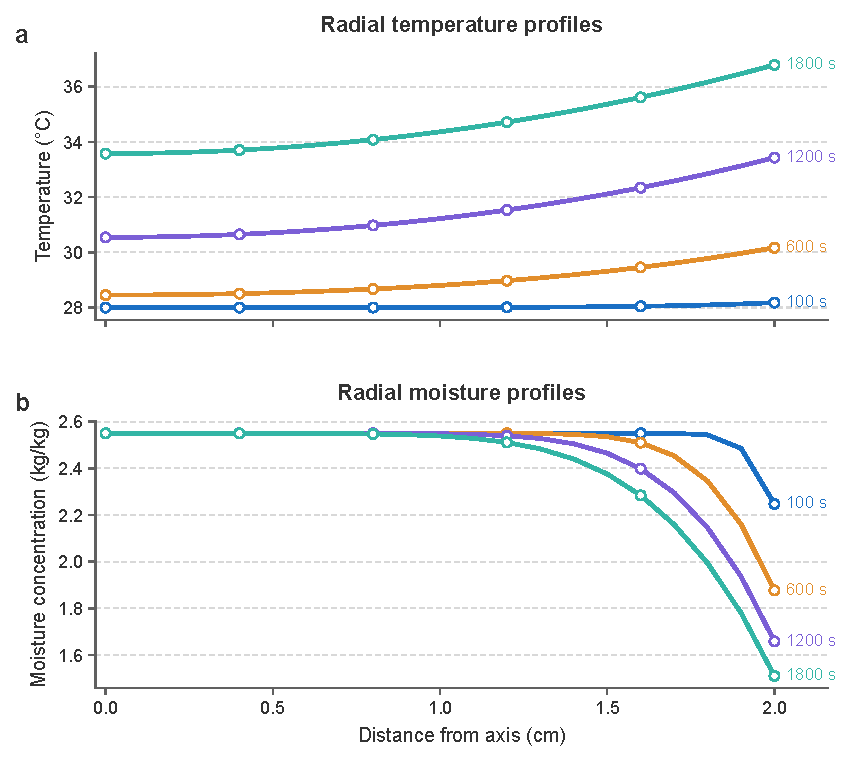
\includegraphics[width=0.92\linewidth]{q1/q1_radial_profiles.pdf}
\caption{问题一典型时刻的径向温度与干基含水率剖面}
\label{fig:q1-radial-profiles}
\end{figure}

\begin{figure}[htbp]
\centering
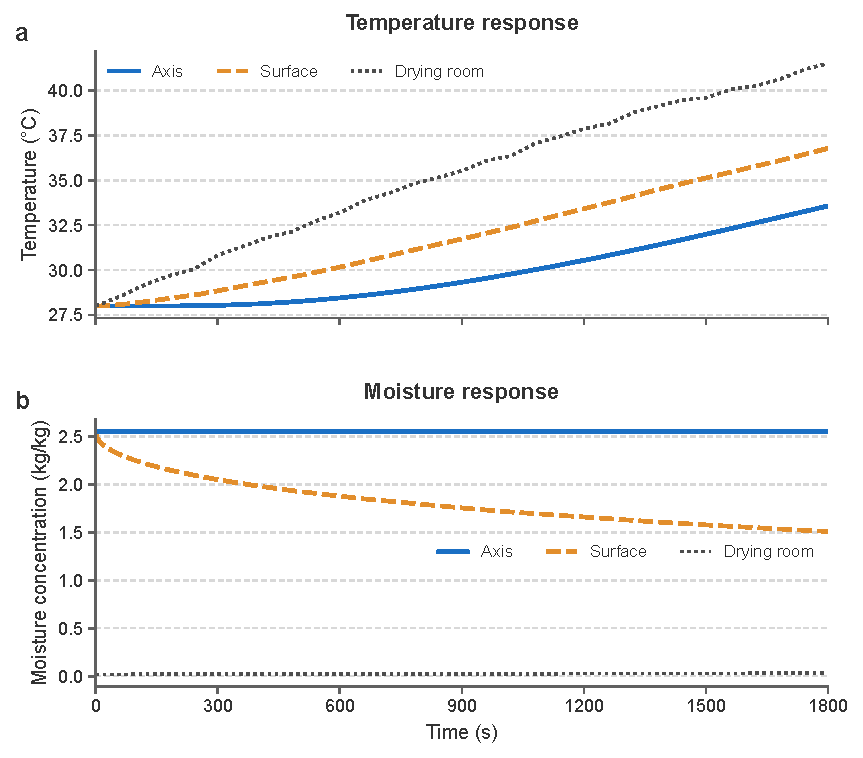
\includegraphics[width=0.92\linewidth]{q1/q1_center_surface_response.pdf}
\caption{问题一轴线、表面与烘房环境的温度和含水率响应}
\label{fig:q1-center-surface}
\end{figure}

\subsubsection{数值检验与适用范围}

首先进行网格加密检验，以判断空间离散误差是否会改变表格结果。相邻网格 $N=1281$ 与 $N=2561$ 在完整输出网格上的最大温度差为 $8.113\times10^{-6}\,{}^\circ\mathrm{C}$，最大含水率差为 $7.294\times10^{-5}\,\mathrm{kg/kg}$；在表\ref{tab:q1-moisture}的取值点上，含水率最大差为 $5.425\times10^{-6}\,\mathrm{kg/kg}$。各级网格差异随加密总体下降，因此本文结果在所用空间离散下具有稳定性。这里的检验用于评价空间离散误差，不将结果表述为严格的四位小数收敛证明。

其次进行时间积分容差敏感性检验。在 $N=2561$ 下收紧 BDF 容差后，表格点温度最大变化为 $6.669\times10^{-6}\,{}^\circ\mathrm{C}$，含水率最大变化为 $8.405\times10^{-8}\,\mathrm{kg/kg}$，说明正式表格结果对时间积分精度不敏感。

最后对控制体方程进行全域积分，比较储量变化率和外表面边界通量。瞬时平衡残差用于检查有限体积通量求和的一致性；以每 $1\,\mathrm{s}$ 输出作梯形积分后，温度能量平衡和水分模型积分平衡的累计相对残差分别为 $1.796\times10^{-7}$ 和 $1.861\times10^{-6}$，均不超过 $2\times10^{-6}$。同时，所有输出均为有限数，无负含水率，未发现明显非物理振荡或异常极值。上述检查分别对应空间离散、时间积分和边界通量一致性，不能替代实验验证，也不用于证明物理模型绝对正确。

从特征时间看，热扩散率约为 $1.69\times10^{-7}\,\mathrm{m^2/s}$，对应径向热扩散时间约 $2.37\times10^3\,\mathrm{s}$；初始含水率下水分扩散系数约为 $4.94\times10^{-9}\,\mathrm{m^2/s}$，对应时间约 $8.1\times10^4\,\mathrm{s}$。前者与 $1800\,\mathrm{s}$ 同量级，后者显著更长，因此“温度变化已进入内部，而水分变化主要集中在表面”的结果具有时间尺度上的解释。该解释适用于本题给定的几何、物性和 $0$--$1800\,\mathrm{s}$ 环境数据范围。

\subsubsection{问题一小结}

本文建立了固定尺寸长圆柱的一维径向温度—水分解耦模型，并用守恒有限体积法求得预热平衡阶段的时空分布。计算结果表明，1800 s 内药材表面升温和失水均明显快于中心，温度场逐步向内部传播，而水分场仍受内部扩散限制。现有表格、图件和数值检验共同支持将该结果作为问题一的正式结果，并为后续引入变物性和全过程模型提供固定物性基准及数值离散参照。

\section{问题二：变物性耦合传热传质模型}

问题二将问题一的时间窗口由 $1800\,\mathrm{s}$ 扩展到 $10800\,\mathrm{s}$，要求在相同径向位置给出前三小时的温度和含水率演化。问题一中物性参数取常数，温度场与水分场可以解耦；问题二根据附录3引入含水率相关的密度、比热容和导热系数，并使水分扩散系数同时依赖含水率和温度。因此，本问继承问题一的固定尺寸一维径向几何、初始条件、环境数据插值和第三类表面边界，但将两个独立方程升级为温度—水分双向参数耦合系统。

药材仍近似为半径 $R=0.02\,\mathrm{m}$、长度 $L=0.25\,\mathrm{m}$ 的轴对称长圆柱，仅描述 $r\in[0,R]$ 上的径向过程。该模型主要适用于圆柱主体区域，忽略周向和轴向变化，不能刻画靠近两端端面的局部轴向效应。问题二从题目给定的 $t=0$ 状态重新计算，不续接问题一在 $1800\,\mathrm{s}$ 时的数值状态，也暂不考虑尺寸收缩。由于从 $t=0$ 起即采用附录3变物性重新计算，其 $1800\,\mathrm{s}$ 状态不要求与问题一采用附录2物性所得结果一致。

\subsection{变物性热质耦合模型的建立}

问题二需要同时描述热量储存、热传导和水分扩散。令 $T(r,t)$ 为摄氏温度，$C(r,t)$ 为干基含水率，则温度场满足
\begin{equation}
\rho(C)c_p(C)\frac{\partial T}{\partial t}
=\frac{1}{r}\frac{\partial}{\partial r}
\left[rk(C)\frac{\partial T}{\partial r}\right],
\qquad 0<r<R,
\label{eq:q2-temperature}
\end{equation}
水分场满足
\begin{equation}
\frac{\partial C}{\partial t}
=\frac{1}{r}\frac{\partial}{\partial r}
\left[rD(C,T)\frac{\partial C}{\partial r}\right],
\qquad 0<r<R.
\label{eq:q2-moisture}
\end{equation}

式\eqref{eq:q2-temperature}中的储热系数、导热系数和式\eqref{eq:q2-moisture}中的扩散系数均随状态变化。附录3给出的关系为
\begin{equation}
\rho(C)=650+128C,
\label{eq:q2-density}
\end{equation}
\begin{equation}
c_p(C)=1450+2736\frac{C}{C+1},
\qquad
k(C)=0.21+0.38\frac{C}{C+1},
\label{eq:q2-properties}
\end{equation}
\begin{equation}
D(C,T)=2.4\times10^{-3}
\exp\left(-\frac{0.45}{C}\right)
\exp\left(-\frac{3850}{T_K}\right)\,\mathrm{m^2/s}.
\label{eq:q2-diffusivity}
\end{equation}

$T$、$T_a$ 和 $T_s$ 均为摄氏温度；Arrhenius 关系采用绝对温度，记
\begin{equation}
T_K=T+273.15,
\label{eq:q2-kelvin}
\end{equation}
并在式\eqref{eq:q2-diffusivity}中使用 $T_K$。由式\eqref{eq:q2-density}--\eqref{eq:q2-diffusivity}可见，$C$ 会改变 $\rho$、$c_p$、$k$ 和 $D$，而 $T$ 会通过 $T_K$ 改变 $D$，求解时需要同步更新物性参数，以反映两个场之间的相互影响。

取题目给定的初始温度和含水率：
\begin{equation}
T(r,0)=28\,{}^\circ\mathrm{C},
\qquad
C(r,0)=2.55\,\mathrm{kg/kg},
\qquad 0\le r\le R.
\label{eq:q2-initial}
\end{equation}

\subsection{模型的求解}

径向正方向由轴线指向药材表面。在 $r=0$ 处采用轴对称零通量条件：
\begin{equation}
\left.\frac{\partial T}{\partial r}\right|_{r=0}=0,
\qquad
\left.\frac{\partial C}{\partial r}\right|_{r=0}=0.
\label{eq:q2-center-bc}
\end{equation}

在 $r=R$ 处，本文采用第三类对流边界：
\begin{equation}
-k(C_s)\left.\frac{\partial T}{\partial r}\right|_{r=R}
=h\bigl(T_s-T_a(t)\bigr),
\label{eq:q2-thermal-bc}
\end{equation}
\begin{equation}
-D(C_s,T_s)\left.\frac{\partial C}{\partial r}\right|_{r=R}
=h_m\bigl(C_s-C_a(t)\bigr),
\label{eq:q2-moisture-bc}
\end{equation}
其中 $T_s=T(R,t)$、$C_s=C(R,t)$。附录3没有重新给出表面对流换热系数和传质系数，因此本文补充假设继续沿用问题一的 $h=25\,\mathrm{W/(m^2\cdot K)}$ 和 $h_m=8\times10^{-7}\,\mathrm{m/s}$。

附件1共有 $0$--$14400\,\mathrm{s}$ 的241组环境记录；问题二使用其中 $0$--$10800\,\mathrm{s}$ 的181组记录。对相邻数据点之间的烘房温度 $T_a(t)$ 和水分浓度 $C_a(t)$ 采用分段线性插值，不进行平滑或外推。控制方程在整个计算时段内保持一致。

\subsection{结果的得出与分析}

将 $[0,R]$ 均匀划分为 $N$ 个环形控制体，在每个控制体上对式\eqref{eq:q2-temperature}和式\eqref{eq:q2-moisture}积分。中心界面通量严格置零；内部界面上的 $k$ 和 $D$ 均取相邻控制体物性的调和平均，使相邻控制体共享同一界面通量，保持离散通量的守恒性。水分方程始终保留 $\nabla\cdot(D\nabla C)$ 的变系数形式。

外表面不直接把最外控制体中心值作为 $T_s$ 或 $C_s$。对温度，将最外控制体中心至真实表面的半网格导热关系与式\eqref{eq:q2-thermal-bc}联立；对水分，将半网格扩散关系与式\eqref{eq:q2-moisture-bc}联立，并在表面扩散系数中使用当前 $C_s$ 和 $T_s+273.15$。水分表面方程可能存在退化数学根，数值上沿最外控制体浓度到环境浓度的连续方向搜索首个物理解，以保持网格细化时表面状态与内部状态相容。该选根策略用于维持边界求解的连续性，不据此断言基准计算中已发生多根异常。

将温度和水分控制体未知量拼接为
\begin{equation}
\boldsymbol y(t)=
\bigl[T_1,\ldots,T_N,C_1,\ldots,C_N\bigr]^{\mathsf T},
\label{eq:q2-state}
\end{equation}
得到维数为 $2N$ 的刚性常微分方程组。采用 BDF 方法同步积分；每次计算右端项时，根据当前状态实时更新 $\rho(C)$、$c_p(C)$、$k(C)$ 和 $D(C,T)$，不冻结旧时刻物性，也不进行温度—水分顺序分裂。计算结果再通过关于 $r^2$ 的两点线性外推得到轴线值，并用 PCHIP 重构到题目要求的径向位置。

正式计算取 $N=2561$，设置 $\mathrm{rtol}=10^{-8}$、温度绝对容差 $10^{-10}$、水分绝对容差 $10^{-11}$、最大内部时间步长 $10\,\mathrm{s}$。未舍入结果保留 $t=0,1,\ldots,10800\,\mathrm{s}$ 和 $r=0,0.001,\ldots,0.020\,\mathrm{m}$；题目指定结果表从 $t=1\,\mathrm{s}$ 开始填写，并将数值保留四位小数。

\subsubsection{计算结果与规律分析}

取 $t=0.5,1.0,\ldots,3.0\,\mathrm{h}$ 及 $r=0,0.5,\ldots,2.0\,\mathrm{cm}$，所得温度与干基含水率分别列于表\ref{tab:q2-temperature}和表\ref{tab:q2-moisture}。

\begin{table}[H]
\centering
\caption{不同时间与径向位置的温度}
\label{tab:q2-temperature}
\zihao{-5}
\begin{tabular}{@{}crrrrr@{}}
\toprule
\multicolumn{6}{c}{$T(r,t)/{}^\circ\mathrm{C}$}\\
\midrule
$t/\mathrm{h}$ & $r=0\,\mathrm{cm}$ & $r=0.5\,\mathrm{cm}$ & $r=1.0\,\mathrm{cm}$ & $r=1.5\,\mathrm{cm}$ & $r=2.0\,\mathrm{cm}$ \\
\midrule
0.5 & 32.1892 & 32.3821 & 32.9659 & 33.9608 & 35.4130 \\
1.0 & 40.3816 & 40.5536 & 41.0605 & 41.8782 & 42.9976 \\
1.5 & 45.8468 & 45.9348 & 46.1930 & 46.6051 & 47.1401 \\
2.0 & 48.4502 & 48.4881 & 48.5984 & 48.7736 & 49.0033 \\
2.5 & 49.4670 & 49.4792 & 49.5136 & 49.5653 & 49.6609 \\
3.0 & 49.8495 & 49.8553 & 49.8746 & 49.9101 & 49.9664 \\
\bottomrule
\end{tabular}
\end{table}

\begin{table}[H]
\centering
\caption{不同时间与径向位置的干基含水率}
\label{tab:q2-moisture}
\zihao{-5}
\begin{tabular}{@{}crrrrr@{}}
\toprule
\multicolumn{6}{c}{$C(r,t)/(\mathrm{kg/kg})$}\\
\midrule
$t/\mathrm{h}$ & $r=0\,\mathrm{cm}$ & $r=0.5\,\mathrm{cm}$ & $r=1.0\,\mathrm{cm}$ & $r=1.5\,\mathrm{cm}$ & $r=2.0\,\mathrm{cm}$ \\
\midrule
0.5 & 2.5499 & 2.5489 & 2.5256 & 2.3257 & 1.6486 \\
1.0 & 2.5257 & 2.4948 & 2.3578 & 2.0230 & 1.4711 \\
1.5 & 2.3861 & 2.3256 & 2.1344 & 1.8020 & 1.3476 \\
2.0 & 2.1709 & 2.1084 & 1.9236 & 1.6259 & 1.2311 \\
2.5 & 1.9566 & 1.9006 & 1.7360 & 1.4720 & 1.1166 \\
3.0 & 1.7662 & 1.7165 & 1.5702 & 1.3333 & 1.0081 \\
\bottomrule
\end{tabular}
\end{table}

计算结果显示，温度趋于均匀的速度明显快于含水率。$0.5\,\mathrm{h}$ 时，轴线与表面温度分别为 $32.1892\,{}^\circ\mathrm{C}$ 和 $35.4130\,{}^\circ\mathrm{C}$；至 $3\,\mathrm{h}$，两者分别为 $49.8495\,{}^\circ\mathrm{C}$ 和 $49.9664\,{}^\circ\mathrm{C}$，温差缩小至约 $0.12\,{}^\circ\mathrm{C}$。相比之下，$3\,\mathrm{h}$ 时轴线与表面含水率仍分别为 $1.7662\,\mathrm{kg/kg}$ 和 $1.0081\,\mathrm{kg/kg}$，内部尚保留明显的水分梯度。

% 首次引用、图片和题注作为一个非浮动块排版，防止图文分离。
\par\addvspace{\medskipamount}
\noindent\begin{minipage}{\linewidth}
\setlength{\parindent}{2em}
六个时刻的径向分布如图\ref{fig:q2-radial-profiles}所示，可进一步比较温度与含水率由表及里的响应差异。
\par\smallskip
\centering
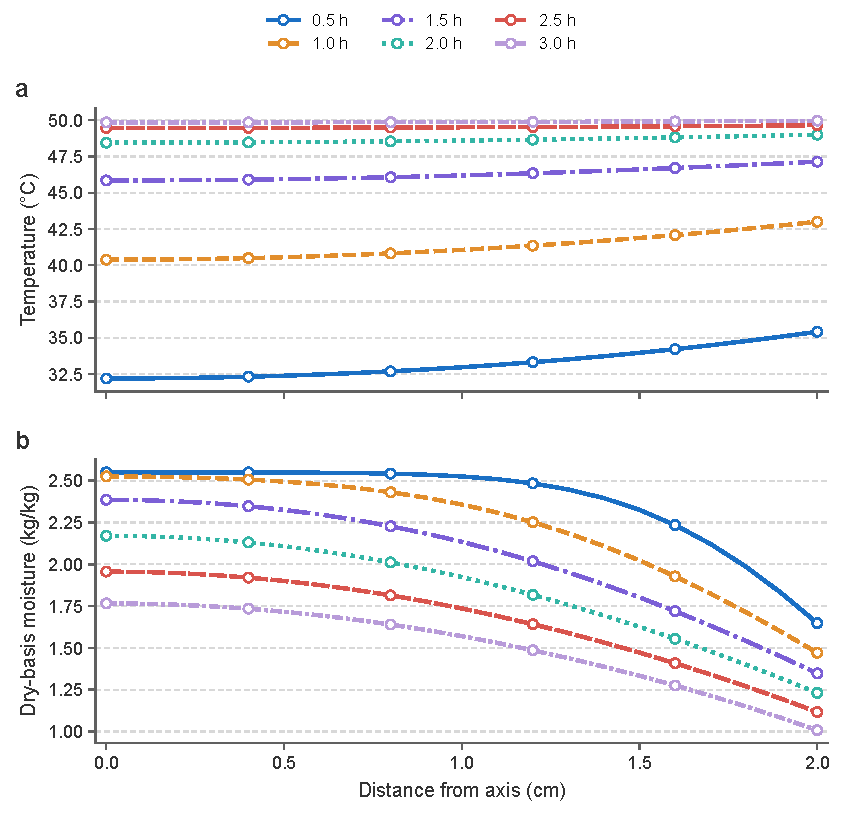
\includegraphics[width=0.78\linewidth]{q2/q2_radial_profiles.pdf}
\captionof{figure}{不同时刻的径向温度与含水率分布}
\label{fig:q2-radial-profiles}
\end{minipage}
\par\addvspace{\medskipamount}

温度剖面随时间逐渐变平，而含水率剖面持续表现为内部高、表面低。初期表面先失水，轴线含水率变化较小；随后内部水分向表面迁移，轴线含水率才逐步下降。以初始物性估算，热扩散率 $\alpha_0=k(C_0)/[\rho(C_0)c_p(C_0)]\approx1.4483\times10^{-7}\,\mathrm{m^2/s}$，水分扩散系数 $D_0\approx5.6417\times10^{-9}\,\mathrm{m^2/s}$，相应的径向特征时间 $R^2/\alpha_0$ 与 $R^2/D_0$ 分别约为 $2762\,\mathrm{s}$ 和 $70901\,\mathrm{s}$。两者的差异与前三小时内温度趋于均匀、含水率仍明显不均的计算结果相符。

\par\addvspace{\medskipamount}
\noindent\begin{minipage}{\linewidth}
\setlength{\parindent}{2em}
为考察温度与含水率对水分迁移速率的共同影响，图\ref{fig:q2-diffusivity}给出了轴线和表面处水分扩散系数的变化。
\par\smallskip
\centering
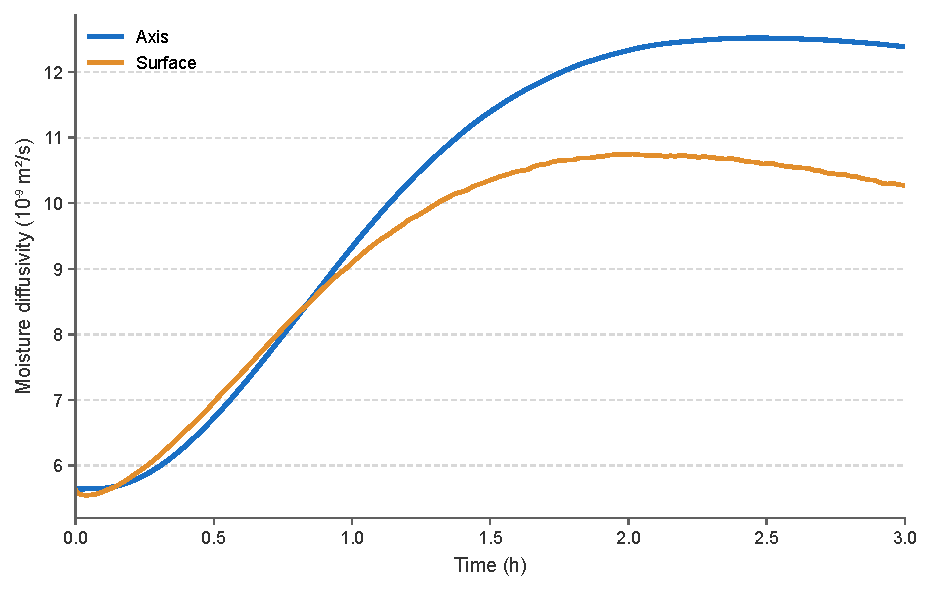
\includegraphics[width=0.82\linewidth]{q2/q2_diffusivity_timeseries.pdf}
\captionof{figure}{轴线与表面水分扩散系数的变化}
\label{fig:q2-diffusivity}
\end{minipage}
\par\addvspace{\medskipamount}

由式\eqref{eq:q2-diffusivity}可知，在另一变量不变时，升温使 $D$ 增大，含水率下降则使 $D$ 减小。计算过程中，两处的扩散系数均表现为先增大、后缓慢减小；表面回落早于轴线。这说明前期升温的促进作用占优，后期温升趋缓，失水的抑制作用逐渐显现。因而，含水率变化不仅是扩散过程的结果，也会通过物性变化反过来影响后续传热与传质。

\subsubsection{数值检验与适用范围}

首先进行网格加密检验。相邻网格 $N=1281$ 和 $N=2561$ 在完整输出网格上的最大温度差为 $3.55\times10^{-5}\,{}^\circ\mathrm{C}$，最大含水率差为 $5.96\times10^{-5}\,\mathrm{kg/kg}$；在表\ref{tab:q2-temperature}和表\ref{tab:q2-moisture}取值点上的最大差分别为 $4.79\times10^{-6}\,{}^\circ\mathrm{C}$ 和 $2.10\times10^{-7}\,\mathrm{kg/kg}$。温度与含水率的最大差异分别出现在 $t=9900\,\mathrm{s}$ 和 $t=1\,\mathrm{s}$ 的表面位置。表列时刻从 $1800\,\mathrm{s}$ 起，其取值对网格加密的变化较小。

其次进行 BDF 容差敏感性检验。在 $N=2561$ 下将参数收紧为 $\mathrm{rtol}=10^{-10}$、温度和水分绝对容差分别为 $10^{-12}$ 和 $10^{-13}$、最大步长为 $2\,\mathrm{s}$ 后，表格点温度最大变化为 $1.30\times10^{-5}\,{}^\circ\mathrm{C}$，含水率最大变化为 $1.81\times10^{-8}\,\mathrm{kg/kg}$，说明表格结果对时间积分设置不敏感。

最后对有限体积控制体进行全域积分平衡检查。在选取的10个检验时刻，方程左端项的体积分与表面边界通量之间的最大相对残差分别为 $2.55\times10^{-16}$（温度）和 $2.16\times10^{-16}$（含水率输运）。基于每 $1\,\mathrm{s}$ 未舍入状态的累计积分，在 $10800\,\mathrm{s}$ 终点的温度路径积分相对残差为 $4.12\times10^{-8}$，含水率输运积分相对残差为 $3.87\times10^{-7}$。由于 $\rho c_p$ 随含水率变化，热量平衡按 $\int_0^t\int_V \rho c_p(\partial T/\partial t)\,\mathrm dV\,\mathrm d\tau$ 计算；含水率平衡则比较 $\int_V C\,\mathrm dV$ 的变化与累计边界通量。这两项检查反映了所建方程的离散一致性。

所有正式输出均为有限值，含水率保持为正，未发现明显空间锯齿或异常极值。后期约 $2.9\,\mathrm{h}$ 的近表面温度剖面出现小幅非单调响应，与附件1环境温度的波动相对应；因此，径向温度在全过程中并非严格单调。上述网格、容差和积分平衡检查用于说明数值离散稳定性与边界通量一致性，不能替代实验验证，也不能单独证明物理模型与真实药材完全一致。

\subsubsection{问题二小结}

本文在问题一固定几何模型的基础上引入含水率相关物性和温度相关扩散系数，建立了温度—水分双向参数耦合模型。结果表明，前三小时内药材温度迅速接近烘房环境，水分由内部向表面迁移，轴线失水响应明显滞后。网格加密、时间容差和全域积分平衡检查支持当前表格结果的数值稳定性；该模型为后续延长计算时段、确定达标时间提供了基础。

\section{问题三：达标烘干时间与全域终止判定}

问题三要求确定药材全域水分浓度降至 $0.15\,\mathrm{kg/kg}$ 所需的烘干时间，并给出题目指定时刻和径向位置的水分浓度。与问题二相比，本问的主要变化是计算时段从前三小时延长到达标时刻，且判停条件作用于整个药材区域，而不是某一个观测位置。因此，本问继承问题二的轴对称长圆柱几何、变物性温度—水分耦合方程、第三类表面边界和守恒有限体积离散，只扩展计算时域并增加全域终止事件。

药材仍近似为半径 $R=0.02\,\mathrm{m}$、长度 $L=0.25\,\mathrm{m}$ 的轴对称长圆柱，仅描述 $r\in[0,R]$ 上的径向传热传质过程。问题三从题目给定的均匀初始状态重新计算，不把问题二的终态作为初值。附件1在 $0$--$14400\,\mathrm{s}$ 内的环境温度和环境水分浓度采用分段线性插值；超过该数据范围后，本文将两项环境量保持为附件末值 $T_a=50.165\,{}^\circ\mathrm{C}$ 和 $C_a=0.04986\,\mathrm{kg/kg}$。这是题目数据终止后的补充边界假设。

\subsection{全域阈值事件模型的建立}

问题三沿用问题二的温度—水分耦合模型。令 $T(r,t)$ 为摄氏温度，$C(r,t)$ 为干基水分浓度，则温度场和水分场分别满足
\begin{equation}
\rho(C)c_p(C)\frac{\partial T}{\partial t}
=\frac{1}{r}\frac{\partial}{\partial r}
\left[rk(C)\frac{\partial T}{\partial r}\right],
\qquad 0<r<R,
\label{eq:q3-temperature}
\end{equation}
\begin{equation}
\frac{\partial C}{\partial t}
=\frac{1}{r}\frac{\partial}{\partial r}
\left[rD(C,T)\frac{\partial C}{\partial r}\right],
\qquad 0<r<R.
\label{eq:q3-moisture}
\end{equation}

式\eqref{eq:q3-temperature}--\eqref{eq:q3-moisture}中的物性关系与问题二相同，特别是水分扩散系数中的 Arrhenius 温度单独按
\begin{equation}
T_K=T+273.15
\label{eq:q3-kelvin}
\end{equation}
换算为开尔文温度。正文中的 $T$、$T_a$ 和 $T_s$ 始终表示摄氏温度。该模型仍不显式加入收缩、吸附等温线和蒸发潜热；这些处理是沿用问题二的建模简化，不表示相应物理机制在实际过程中不存在。

径向正方向由轴线指向表面。轴线采用零通量条件，外表面采用问题二中的第三类对流边界：
\begin{equation}
\left.\frac{\partial T}{\partial r}\right|_{r=0}=0,
\qquad
\left.\frac{\partial C}{\partial r}\right|_{r=0}=0,
\label{eq:q3-center-bc}
\end{equation}
\begin{equation}
-k(C_s)\left.\frac{\partial T}{\partial r}\right|_{r=R}
=h(T_s-T_a),
\qquad
-D(C_s,T_s)\left.\frac{\partial C}{\partial r}\right|_{r=R}
=h_m(C_s-C_a).
\label{eq:q3-surface-bc}
\end{equation}

为避免只检查某一网格点，定义全域最大水分浓度为
\begin{equation}
C_{\max}(t)=\max\left\{C_{\mathrm{axis}}(t),C_1(t),\ldots,C_N(t),C_s(t)\right\},
\label{eq:q3-cmax}
\end{equation}
其中 $C_i$ 为控制体中心值，$C_s$ 为真实表面值，$C_{\mathrm{axis}}$ 由中心附近关于 $r^2$ 的两点线性外推得到。烘干结束时刻取为 $C_{\max}(t)-0.15$ 第一次由正向负穿越的连续时刻，即
\begin{equation}
C_{\max}(t_e)=0.15\,\mathrm{kg/kg}.
\label{eq:q3-stop}
\end{equation}
事件检测同时覆盖轴线、全部控制体中心和真实表面，因而不预设终点最大值一定位于轴线；事件触发后，再用高分辨率径向重构复核终点位置。

\subsection{模型的求解}

将 $[0,R]$ 划分为 $N$ 个环形控制体，对式\eqref{eq:q3-temperature}和式\eqref{eq:q3-moisture}作守恒积分。内部界面上的 $k$ 和 $D$ 取相邻控制体物性的调和平均，中心界面通量置零；外表面通过半网格传递关系与 Robin 条件联立重构真实表面状态。温度和水分未知量拼接为 $2N$ 维状态向量，采用 BDF 方法同步积分，并在每次计算右端项时更新变物性。空间离散和边界重构均沿用问题二，新增的数值任务是持续积分到式\eqref{eq:q3-stop}触发。

正式长程计算取 $N=2561$，设置温度和水分的绝对容差分别为 $10^{-10}$ 和 $10^{-11}$，相对容差为 $10^{-8}$，BDF 内部最大步长为 $60\,\mathrm{s}$。网格加密、容差敏感性和最大步长对照均使用同一终止事件。结果表按题目要求每 $60\,\mathrm{s}$ 保存一次；\texttt{result3.xlsx} 的完整输出径向位置为 $0,0.1,\ldots,2.0\,\mathrm{cm}$，正文表\ref{tab:q3-moisture}则按题目要求每隔 $0.5\,\mathrm{cm}$ 列示典型时刻结果；水分浓度显示为四位小数。未舍入结果用于数值检验和题目要求的结果表生成。

\subsection{结果的得出与分析}

连续事件检测得到
\begin{equation}
t_e=205818.3509686\,\mathrm{s}=57.1717642\,\mathrm{h}=2.3821568\,\mathrm{d}.
\label{eq:q3-end-time}
\end{equation}
正文将其表述为约 $57.17\,\mathrm{h}$（约 $2.38\,\mathrm{d}$），不把未舍入小数解释为物理精度。终点高分辨率重构的全域最大水分浓度为 $0.1500000\,\mathrm{kg/kg}$，位置在轴线 $r=0$；真实表面水分浓度为 $0.0525359\,\mathrm{kg/kg}$，轴线和表面温度均约为 $50.165\,{}^\circ\mathrm{C}$。

表\ref{tab:q3-moisture}列出题目指定时刻和径向位置的水分浓度。最后一行对应连续事件时刻，用于描述终点径向分布；它不是结果工作簿中的规则采样节点。

\begin{table}[H]
\centering
\caption{问题三典型时刻与径向位置的水分浓度}
\label{tab:q3-moisture}
\zihao{-5}
\begin{tabular}{@{}crrrrr@{}}
\toprule
\multicolumn{6}{c}{$C(r,t)/(\mathrm{kg/kg})$}\\
\midrule
$t/\mathrm{h}$ & $r=0\,\mathrm{cm}$ & $r=0.5\,\mathrm{cm}$ & $r=1.0\,\mathrm{cm}$ & $r=1.5\,\mathrm{cm}$ & $r=2.0\,\mathrm{cm}$ \\
\midrule
6 & 1.0156 & 0.9868 & 0.9006 & 0.7546 & 0.5335 \\
12 & 0.4548 & 0.4418 & 0.4019 & 0.3289 & 0.1639 \\
18 & 0.2979 & 0.2906 & 0.2679 & 0.2247 & 0.0842 \\
24 & 0.2371 & 0.2321 & 0.2161 & 0.1851 & 0.0663 \\
30 & 0.2053 & 0.2013 & 0.1887 & 0.1637 & 0.0597 \\
36 & 0.1854 & 0.1821 & 0.1714 & 0.1501 & 0.0565 \\
42 & 0.1717 & 0.1687 & 0.1593 & 0.1404 & 0.0547 \\
48 & 0.1615 & 0.1588 & 0.1504 & 0.1332 & 0.0536 \\
54 & 0.1535 & 0.1511 & 0.1433 & 0.1275 & 0.0528 \\
57.1718 & 0.1500 & 0.1477 & 0.1402 & 0.1249 & 0.0525 \\
\bottomrule
\end{tabular}
\end{table}

表\ref{tab:q3-moisture}显示，表面水分浓度下降最快，轴线响应最为滞后，径向梯度在后期仍然存在。随着 $C$ 降低，扩散系数中的 $\exp(-0.45/C)$ 因子减小，内部水分迁移逐渐受限，因此最后阶段的浓度下降速度低于早期。仅考察浓度因子 $\exp(-0.45/C)$，其在 $C$ 从 $2.55$ 降至 $0.15\,\mathrm{kg/kg}$ 时由约 $0.838$ 降至 $0.050$，有助于解释后期迁移减慢；这一比较不代表含温度因子的完整扩散系数变化倍数。

曲线在终点附近下降趋缓，但仍在 $t_e$ 处首次穿越 $0.15\,\mathrm{kg/kg}$，说明采用全域最大值而不是表面值作为判停量确实控制了后期内部水分。

\par\addvspace{\medskipamount}
\noindent\begin{minipage}{\linewidth}
\setlength{\parindent}{2em}
为观察全域判停量并确认终止事件位置，图\ref{fig:q3-cmax-threshold}给出 $C_{\max}(t)$ 的时间历程及其与 $0.15\,\mathrm{kg/kg}$ 阈值的交点。
\par\smallskip
\centering
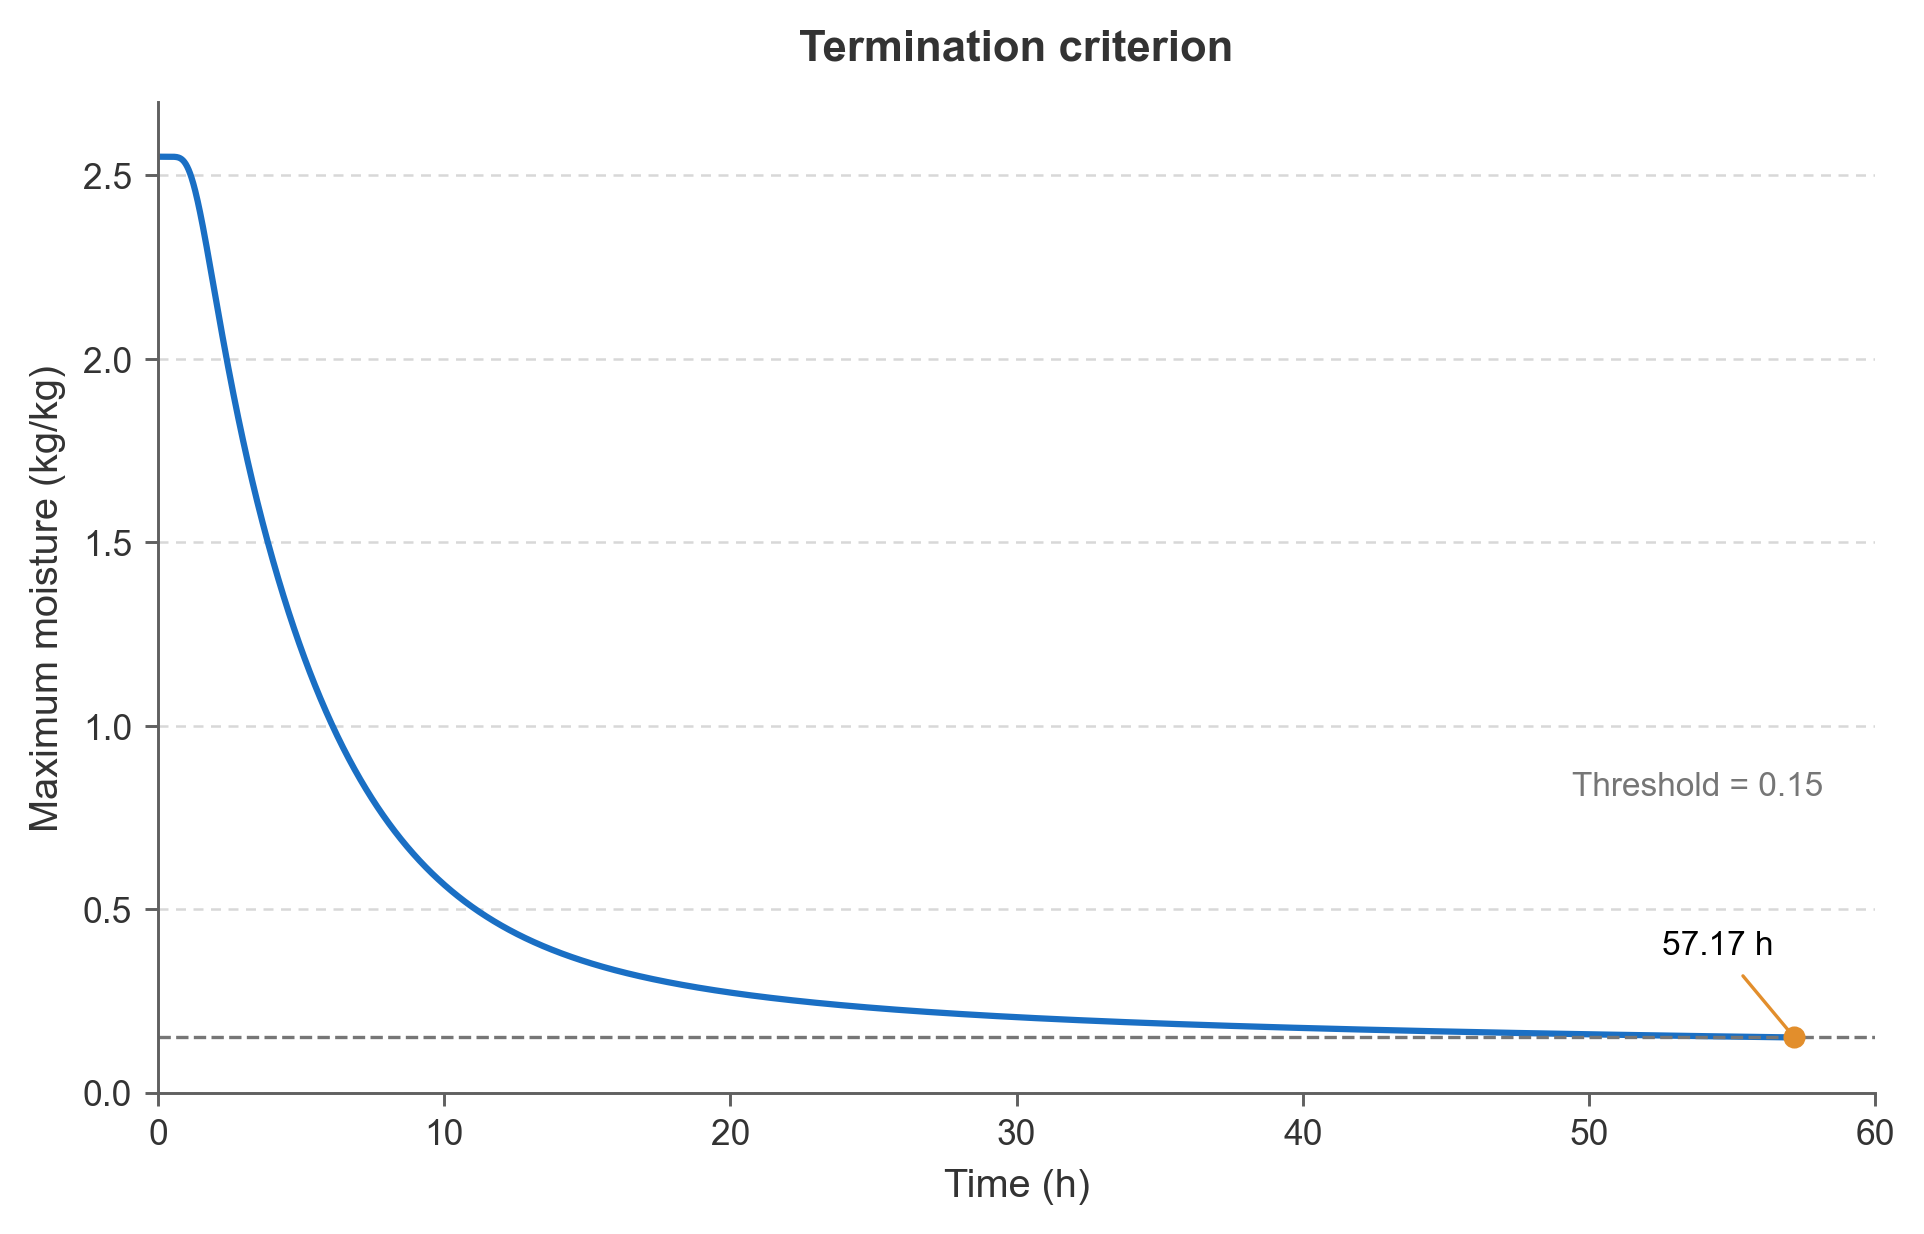
\includegraphics[width=0.82\linewidth]{q3/q3_cmax_threshold.png}
\captionof{figure}{问题三全域最大水分浓度及 $0.15\,\mathrm{kg/kg}$ 终止阈值}
\label{fig:q3-cmax-threshold}
\end{minipage}
\par\addvspace{\medskipamount}

图\ref{fig:q3-spatiotemporal-field}进一步展示水分场的时空变化。橙色等值线表示 $C=0.15\,\mathrm{kg/kg}$，它在终点附近首先接触轴线，和高分辨率终点重构的最大值位置一致。径向剖面图\ref{fig:q3-moisture-profiles}则表明，从早期到终点，表面低浓度区逐步向轴线推进，内部梯度逐渐减小但没有在判停前消失。

\par\addvspace{\medskipamount}
\noindent\begin{minipage}{\linewidth}
\setlength{\parindent}{2em}
时空场用于定位阈值等值线的空间位置，并检验径向剖面随时间的连续变化。
\par\smallskip
\centering
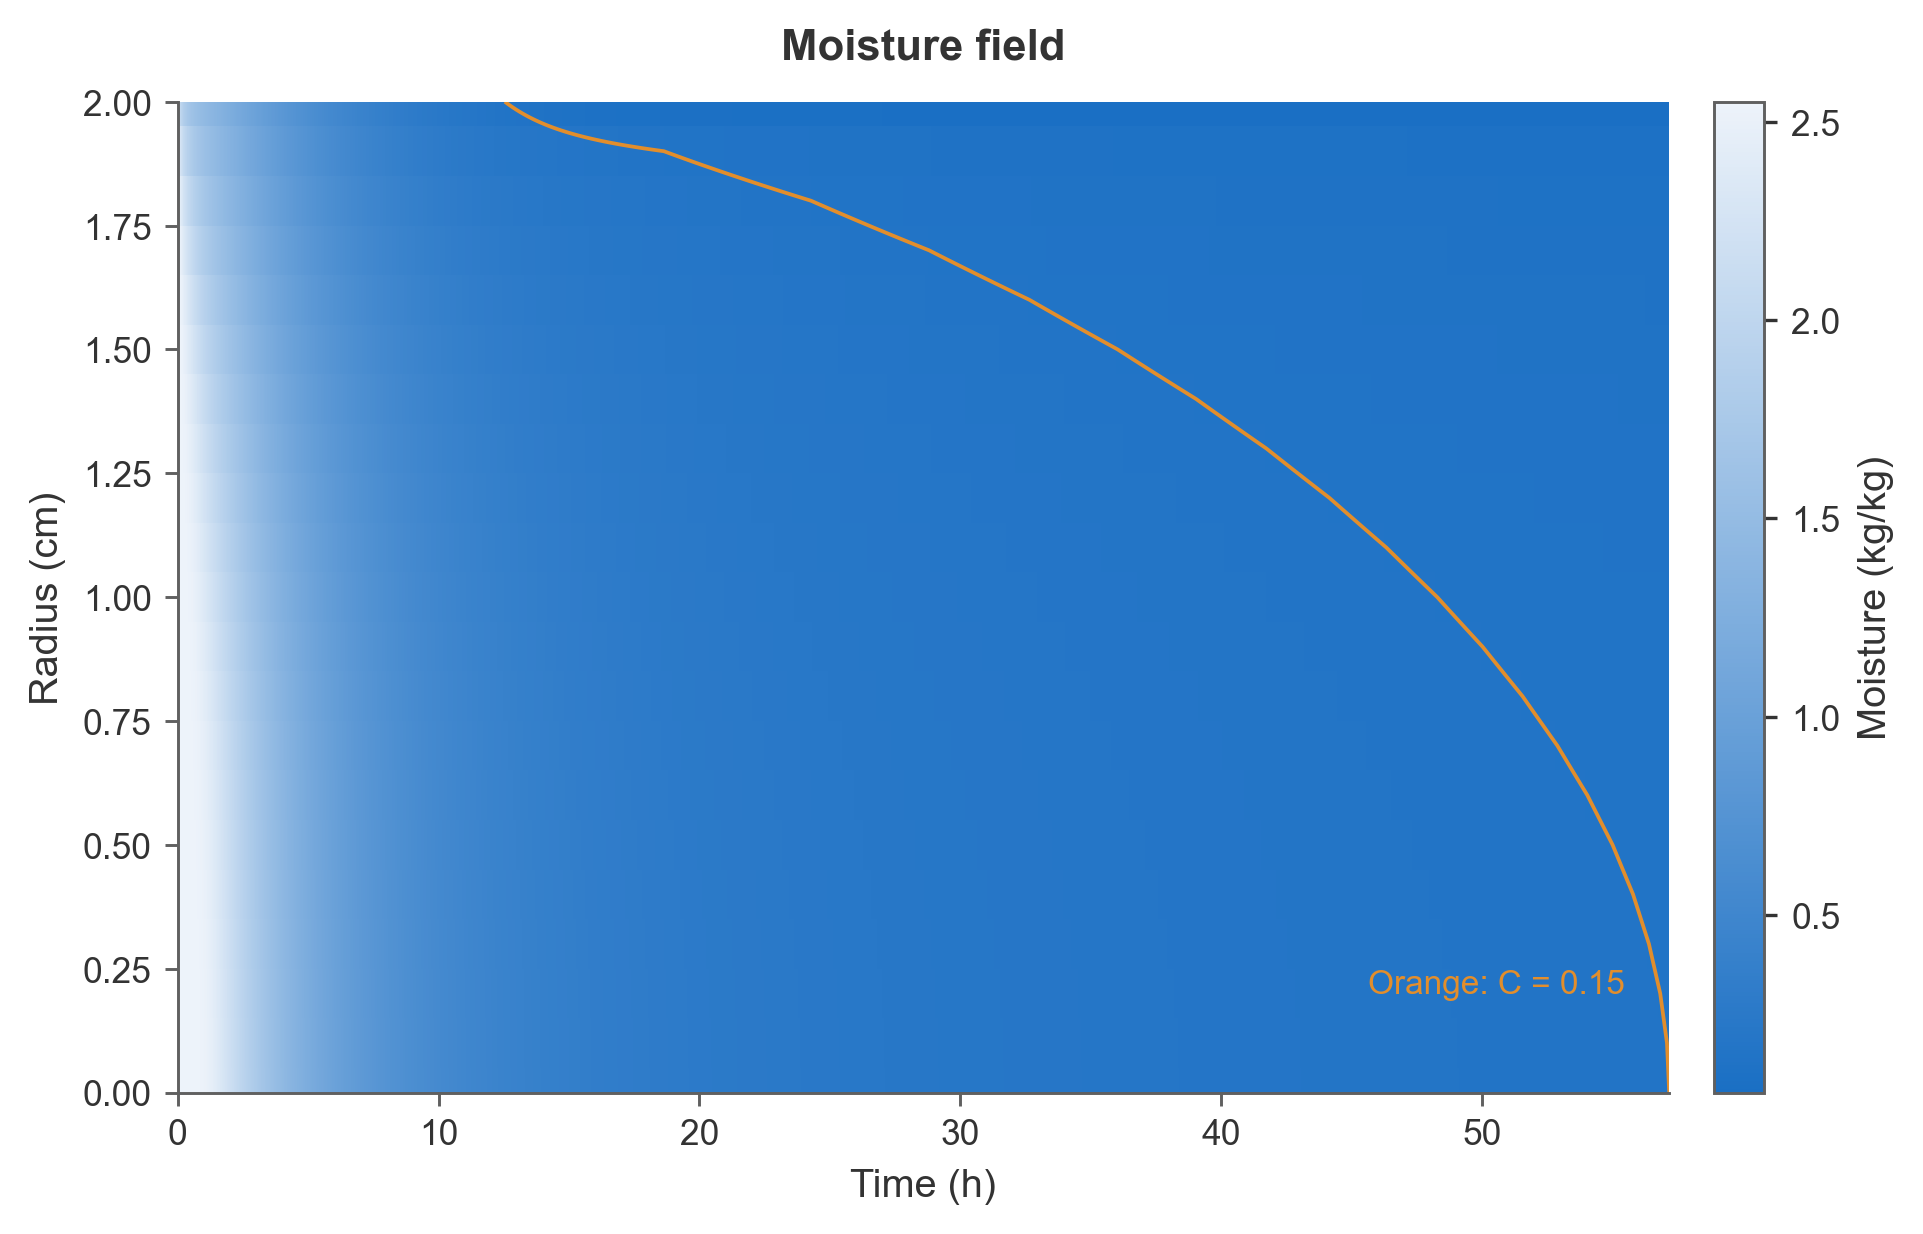
\includegraphics[width=0.82\linewidth]{q3/q3_spatiotemporal_field.png}
\captionof{figure}{问题三水分浓度的时间—半径分布及 $0.15\,\mathrm{kg/kg}$ 等值线}
\label{fig:q3-spatiotemporal-field}
\end{minipage}
\par\addvspace{\medskipamount}

\par\addvspace{\medskipamount}
\noindent\begin{minipage}{\linewidth}
\setlength{\parindent}{2em}
典型时刻的径向剖面如图\ref{fig:q3-moisture-profiles}所示，用于比较表面脱水和内部响应的时间差。
\par\smallskip
\centering
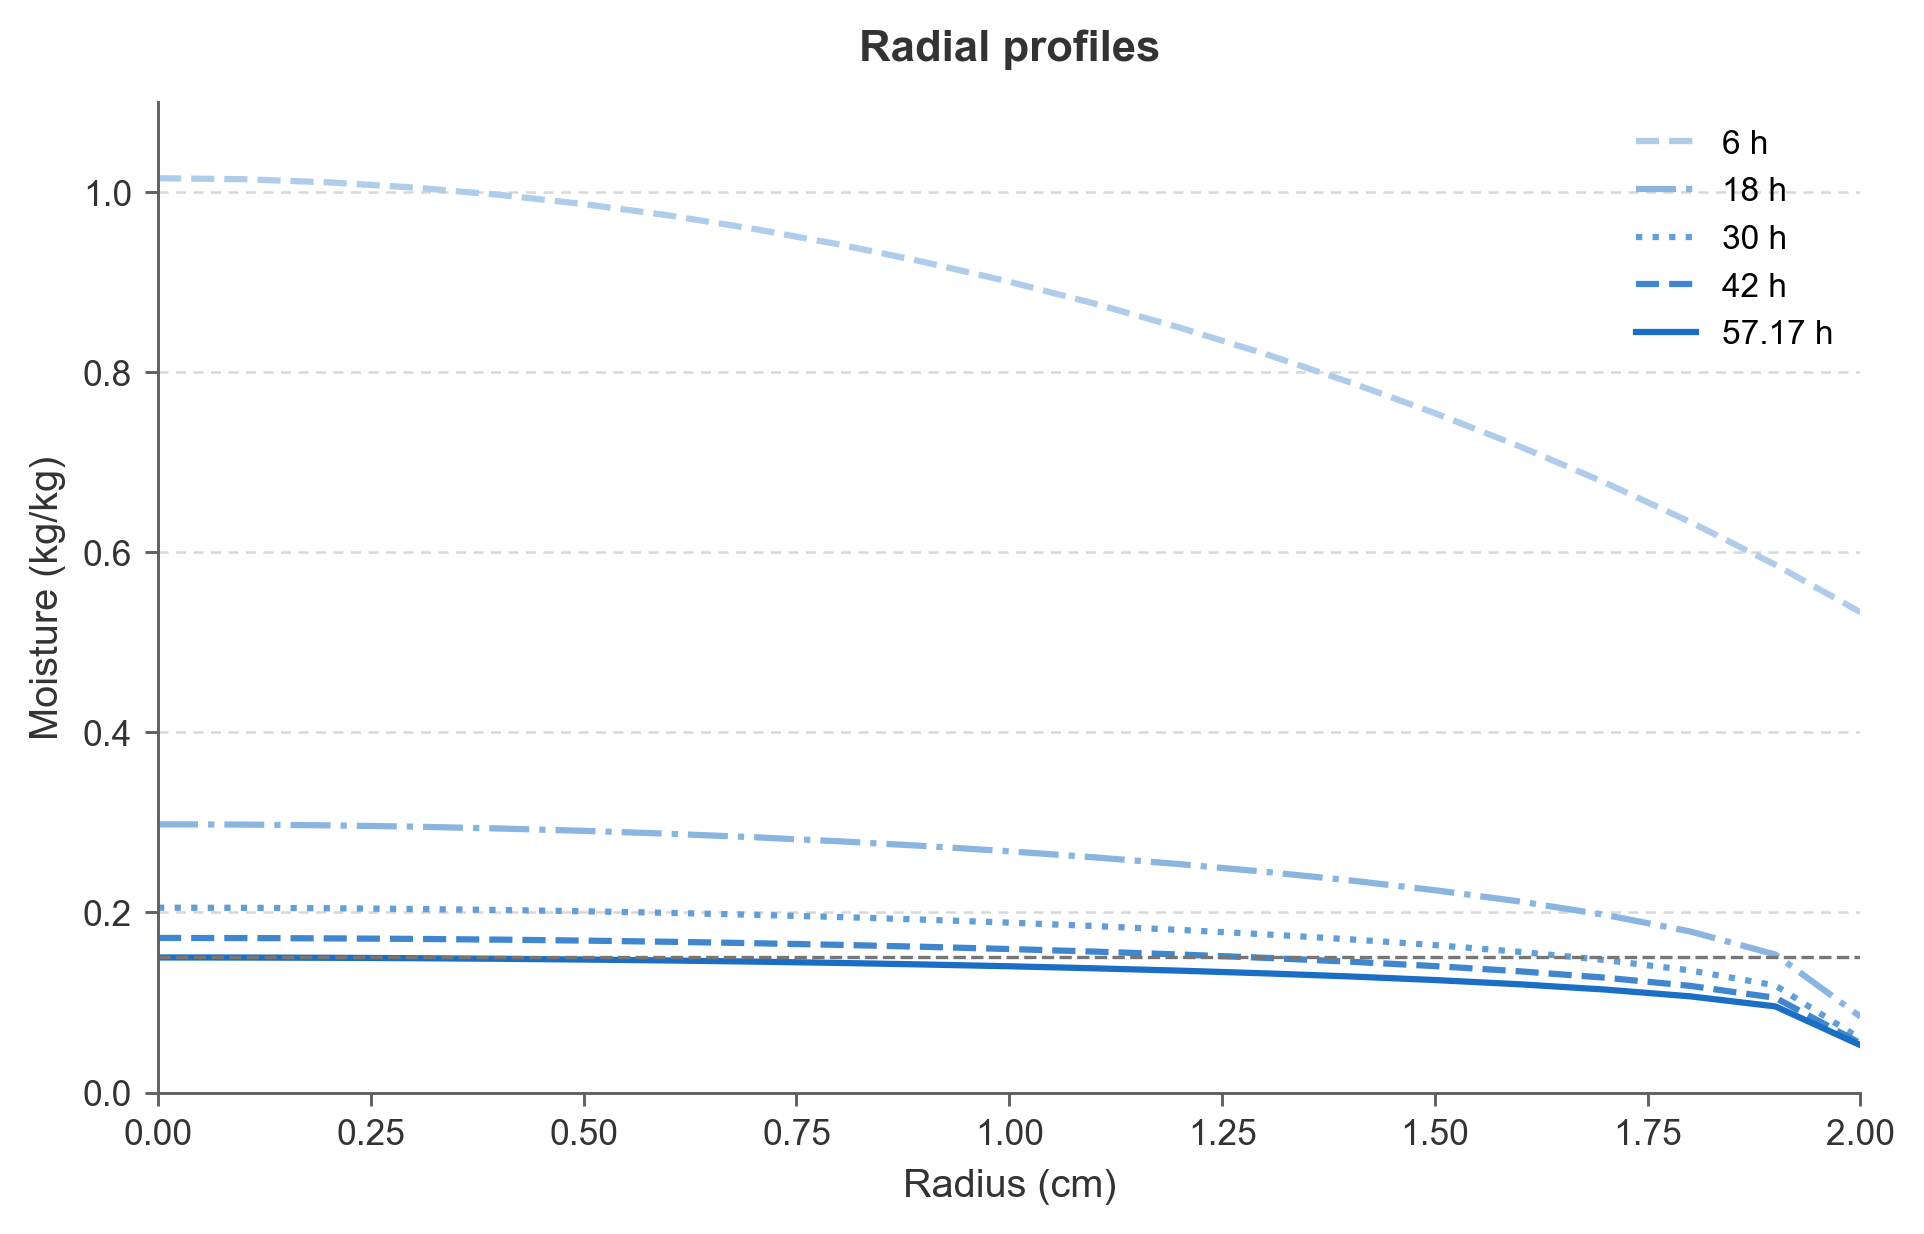
\includegraphics[width=0.82\linewidth]{q3/q3_moisture_profiles.png}
\captionof{figure}{问题三典型时刻的径向水分浓度剖面}
\label{fig:q3-moisture-profiles}
\end{minipage}
\par\addvspace{\medskipamount}

按整数秒解释连续事件时刻，因为 $205818.3509686\,\mathrm{s}$ 位于 $205818\,\mathrm{s}$ 与 $205819\,\mathrm{s}$ 之间，自 $205819\,\mathrm{s}$ 起全域最大水分浓度严格低于阈值。\texttt{result3.xlsx} 按每 $60\,\mathrm{s}$ 保存，因此最后一个不超过 $t_e$ 的规则采样点是 $205800\,\mathrm{s}$；精确事件时刻在表\ref{tab:q3-moisture}中单独给出，不额外写入60 s规则采样序列。

\subsubsection{数值检验与结果稳定性}

首先进行网格加密检验。$N=513,1025,2561$ 时得到的终止时间约为 $57.2067\,\mathrm{h}$、$57.1809\,\mathrm{h}$ 和 $57.1718\,\mathrm{h}$；从 $N=1025$ 到 $N=2561$ 的变化为 $32.9251\,\mathrm{s}$，表\ref{tab:q3-moisture}常规时刻的最大变化降至 $1.84\times10^{-5}\,\mathrm{kg/kg}$。这项检验对应空间离散误差，支持正式网格对表格精度的稳定性。

其次检查时间积分设置。将相对容差从 $10^{-8}$ 放宽至 $10^{-7}$，终止时间仅变化约 $2.8\times10^{-3}\,\mathrm{s}$。

将 BDF 最大内部步长从 $60\,\mathrm{s}$ 改为 $10\,\mathrm{s}$ 后，终止时间仅变化 $0.000399\,\mathrm{s}$，表格值最大差仅为 $4.73\times10^{-9}\,\mathrm{kg/kg}$。这些比较说明结果对时间积分设置不敏感。

再次进行全域积分平衡检查。瞬时有限体积共享通量的积分平衡达到机器精度；由每 $60\,\mathrm{s}$ 保存结果作梯形累计积分，终点累计相对残差为温度 $3.52\times10^{-6}$、水分 $9.34\times10^{-5}$。这里的累计残差用于检验数值离散和边界通量的一致性，不构成实验验证，也不证明物理模型与真实药材完全一致。正式结果均为有限值，水分浓度保持为正；检查未发现明显非物理振荡、负值或异常极值。

问题三在前三小时还与问题二的未舍入结果进行逐点对齐。21 个输出半径上的温度、水分和真实表面状态最大绝对差均为 0，说明延长计算时域没有改变问题二的早期计算结果。该检查属于共享模型实现的一致性核验，不作为独立实验验证。

\subsubsection{环境水分敏感性与模型局限}

附件1数据结束后环境水分浓度的取值会影响后期脱水。将 $14400\,\mathrm{s}$ 之后的 $C_a$ 提高至 $0.07\,\mathrm{kg/kg}$，模型得到烘干时间约为 $57.81\,\mathrm{h}$，比基准情景延长约 $0.63\,\mathrm{h}$。该对照用于说明环境边界变化对后期结果的影响。

\subsubsection{问题三小结}

问题三在问题二耦合模型的基础上延长计算时域，并以全域最大水分浓度定义终止事件。基准环境延拓下，药材达到 $0.15\,\mathrm{kg/kg}$ 全域阈值的时间约为 $57.17\,\mathrm{h}$；终点最大值位于轴线，表面水分浓度已降至约 $0.0525\,\mathrm{kg/kg}$。网格、容差、内部步长、积分平衡和 Q2 早期对齐检查支持该数值结果的稳定性；边界延拓敏感性分析表明，附件数据结束后的环境湿度会影响后期脱水时间。

% 若赛题只有三个问题，可删除或注释下一行。
\section{问题四：考虑径向收缩的耦合传热传质模型}

问题四在问题三全域达标判定的基础上，进一步考虑药材半径随烘干过程变化，并采用附录4的物性关系。新增的困难在于：传递距离随时间缩短，固定观测位置可能移出药材，而物性变化又会改变内部水分迁移速率。因此，本问将移动区域映射到固定材料坐标，在同一框架下求解温度场、水分场与临界烘干时间。

本文保持药材长度 $L=0.25\,\mathrm{m}$ 不变，仅考虑径向收缩，忽略周向和轴向变化，模型适用于圆柱主体区域。初始半径为 $R_0=0.02\,\mathrm{m}$；将附件2的全部半径数据换算为米后，采用保形分段三次 Hermite 插值（PCHIP）构造 $R(t)$\cite{fritsch1980}。计算得到的终止时刻位于附件2时间范围内，无需对半径作外推。几何尺寸完全由 $R(t)$ 确定，经验密度 $\rho(C)$ 仅作为热物性参数，不用于反推半径或体积。

为跟踪收缩中的材料位置，假设药材骨架沿径向随半径同比例缩放，采用移动边界问题中的材料坐标变换\cite{crank1984}，定义
\begin{equation}
\xi=\frac{r}{R(t)},\qquad 0\leq\xi\leq1.
\label{eq:q4-coordinate}
\end{equation}
固定 $\xi$ 对应随骨架运动的材料位置，其物理半径为 $r=\xi R(t)$。以下仍用 $T(\xi,t)$、$C(\xi,t)$ 表示温度和干基水分浓度，时间导数均在固定 $\xi$ 下计算。该处理将材料运动纳入坐标描述，不再另加收缩对流项。

环境边界沿用问题三的处理：附件1在 $0$--$14400\,\mathrm{s}$ 内作分段线性插值，此后保持 $T_a=50.165\,{}^\circ\mathrm{C}$、$C_a=0.04986\,\mathrm{kg/kg}$。长度不变、材料位置同比例缩放及环境末值延拓均为本文的补充假设。

\subsection{移动边界材料坐标模型的建立}

材料坐标将计算区域固定为 $[0,1]$，空间梯度中的长度尺度则由实时半径决定。沿用前两问的扩散与导热描述，控制方程写为
\begin{equation}
\rho(C)c_p(C)\frac{\partial T}{\partial t}
=\frac{1}{R(t)^2\xi}\frac{\partial}{\partial\xi}
\left[\xi k(C)\frac{\partial T}{\partial\xi}\right],
\label{eq:q4-temperature}
\end{equation}
\begin{equation}
\frac{\partial C}{\partial t}
=\frac{1}{R(t)^2\xi}\frac{\partial}{\partial\xi}
\left[\xi D(C,T)\frac{\partial C}{\partial\xi}\right].
\label{eq:q4-moisture}
\end{equation}
其中 $R(t)^{-2}$ 体现收缩对径向传递尺度的影响。温度与水分通过当前状态下的物性相联系，仍同步求解；本文继续忽略蒸发潜热和吸附等温线等机制，作为对实际烘干过程的简化。

附录4给出的物性关系为
\begin{equation}
\begin{aligned}
\rho(C)&=760+90C,\\
c_p(C)&=1850+2150\frac{C}{C+1},\\
k(C)&=0.12+0.20\frac{C}{C+1},\\
D(C,T)&=4.2\times10^{-4}\exp\!\left(-\frac{0.30}{C}\right)
\exp\!\left(-\frac{3850}{T_K}\right),\qquad T_K=T+273.15.
\end{aligned}
\label{eq:q4-properties}
\end{equation}
上述四项物性的单位依次为 $\mathrm{kg/m^3}$、$\mathrm{J/(kg\cdot K)}$、$\mathrm{W/(m\cdot K)}$ 和 $\mathrm{m^2/s}$。$D(C,T)$ 沿用前文的函数记法，但指数项始终代入绝对温度 $T_K$，$T$、$T_a$、$T_s$ 仍表示摄氏温度。

本问从均匀初始状态 $T(\xi,0)=28\,{}^\circ\mathrm{C}$、$C(\xi,0)=2.55\,\mathrm{kg/kg}$ 独立计算。轴线采用零通量条件，真实表面采用第三类对流边界：
\begin{equation}
T_\xi(0,t)=0,\qquad C_\xi(0,t)=0,
\label{eq:q4-axis-bc}
\end{equation}
\begin{equation}
-\frac{k(C_s)}{R(t)}T_\xi(1,t)=h(T_s-T_a),\qquad
-\frac{D(C_s,T_s)}{R(t)}C_\xi(1,t)=h_m(C_s-C_a).
\label{eq:q4-surface-bc}
\end{equation}
这里 $T_s=T(1,t)$、$C_s=C(1,t)$ 均对应实时表面；径向正方向仍由轴线指向表面。附录4未另给边界传递系数，本文沿用 $h=25\,\mathrm{W/(m^2\cdot K)}$ 和 $h_m=8\times10^{-7}\,\mathrm{m/s}$。

\subsection{模型的求解}

在固定材料区间上划分 $N$ 个环形控制体，采用与问题三一致的守恒有限体积法。内部界面物性取调和平均，表面半网格的物理长度随时间更新为 $R(t)\Delta\xi/2$，其中 $\Delta\xi=1/N$。通过半网格传递关系与式\eqref{eq:q4-surface-bc}联立重构表面状态，以避免将最外控制体中心值误作表面值。采用 BDF 同步积分温度和水分，正式计算取 $N=2561$，相对容差 $10^{-8}$，温度和水分绝对容差分别为 $10^{-10}$、$10^{-11}$，最大内部步长为 $60\,\mathrm{s}$。

沿用问题三的全域判停方法，令
\begin{equation}
C_{\max}(t)=\max\{C_{\mathrm{axis}}(t),C_1(t),\ldots,C_N(t),C_s(t)\},
\qquad C_{\max}(t_e)=0.15\,\mathrm{kg/kg}.
\label{eq:q4-event}
\end{equation}
其中轴线值由最内两个控制体中心关于 $\xi^2$ 的两点线性外推得到。连续事件检测寻找阈值函数首次向下穿越零点的时刻，并在终点用 $10001$ 个材料坐标点重构水分场，复核最大值及其位置。

固定物理位置 $r_q$ 的输出通过 $\xi_q=r_q/R(t)$ 定位。当 $r_q>R(t)$ 时，该位置已不属于药材，输出留空；表面列始终取 $\xi=1$，不受固定位置列的变化影响。结果按 $60\,\mathrm{s}$ 的间隔保存，空间插值仅在当前药材域内进行。

\subsection{结果的得出与分析}

连续事件检测得到全域最大水分浓度首次降至阈值的临界时刻为
\begin{equation}
t_e=182956.15\,\mathrm{s}\approx50.82\,\mathrm{h}.
\label{eq:q4-end-time}
\end{equation}
此时药材半径为 $1.2000\,\mathrm{cm}$，最大水分浓度位于轴线，表面水分浓度约为 $0.0525\,\mathrm{kg/kg}$。临界时刻满足等于阈值，其后进入全域严格低于 $0.15\,\mathrm{kg/kg}$ 的区域。按每 $60\,\mathrm{s}$ 保存的最后一个规则采样点为 $182940\,\mathrm{s}$，应与连续事件时刻区分。

表\ref{tab:q4-moisture}给出题目指定时刻及位置的水分浓度，末行单列连续事件时刻。表中“---”表示该固定位置已在当前药材域外，对应结果文件中的空单元格。末列为实时移动表面，不能当作固定半径位置。
\begin{table}[H]
\centering
\caption{径向收缩条件下典型时刻与位置的水分浓度}
\label{tab:q4-moisture}
\zihao{-5}
\begin{tabular}{@{}crrrrrr@{}}
\toprule
\multicolumn{7}{c}{$C(r,t)/(\mathrm{kg/kg})$}\\
\midrule
$t/\mathrm{h}$ & $r=0\,\mathrm{cm}$ & $r=0.5\,\mathrm{cm}$ & $r=1.0\,\mathrm{cm}$ & $r=1.5\,\mathrm{cm}$ & $r=2.0\,\mathrm{cm}$ & $r=R(t)$ \\
\midrule
6 & 1.7164 & 1.5350 & 1.0212 & --- & --- & 0.4215 \\
12 & 0.7340 & 0.6516 & 0.4068 & --- & --- & 0.1666 \\
18 & 0.4065 & 0.3667 & 0.2387 & --- & --- & 0.0888 \\
24 & 0.2837 & 0.2598 & 0.1783 & --- & --- & 0.0671 \\
30 & 0.2253 & 0.2085 & 0.1487 & --- & --- & 0.0593 \\
36 & 0.1920 & 0.1790 & 0.1312 & --- & --- & 0.0558 \\
42 & 0.1706 & 0.1598 & 0.1196 & --- & --- & 0.0539 \\
48 & 0.1556 & 0.1463 & 0.1113 & --- & --- & 0.0529 \\
50.8212 & 0.1500 & 0.1413 & 0.1081 & --- & --- & 0.0525 \\
\bottomrule
\end{tabular}
\end{table}

在 $6\,\mathrm{h}$ 时，半径已缩至 $1.374\,\mathrm{cm}$，因此表中固定 $r=1.5\,\mathrm{cm}$ 和 $r=2.0\,\mathrm{cm}$ 两列均无有效值。到 $30\,\mathrm{h}$，$r=1.0\,\mathrm{cm}$ 处已低于阈值，但轴线仍为 $0.2253\,\mathrm{kg/kg}$；即使在 $48\,\mathrm{h}$，轴线也尚未达标。这说明局部或表面达标不能代替全域终止判定。

\par\addvspace{\medskipamount}
\noindent\begin{minipage}{\linewidth}
\setlength{\parindent}{2em}
图\ref{fig:q4-profiles}以物理半径展示典型时刻的水分分布，各曲线右端即为该时刻的真实表面。
\par\smallskip
\centering
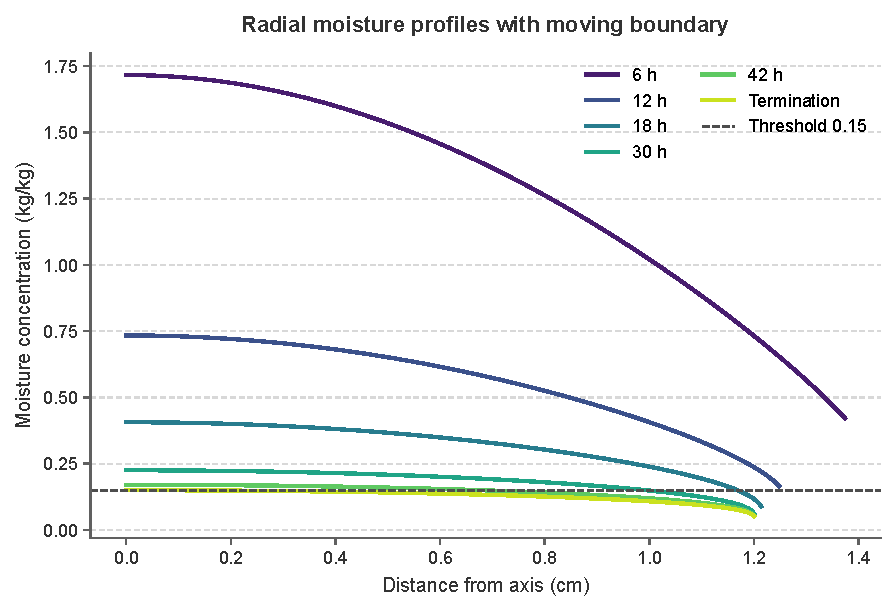
\includegraphics[width=0.78\linewidth]{q4/q4_moving_profiles.pdf}
\captionof{figure}{径向收缩过程中典型时刻的水分浓度剖面}
\label{fig:q4-profiles}
\end{minipage}
\par\addvspace{\medskipamount}

随烘干推进，曲线右端向轴线移动，内部水分浓度逐步下降。后期表面浓度已接近环境值，轴线仍保留较高水分；同时式\eqref{eq:q4-properties}中的水分因子随 $C$ 降低而减小，使内部迁移逐渐放缓。因此，半径缩短虽有利于传递，仍不能消除后期内部水分对烘干时间的控制。

\subsubsection{物性变化与径向收缩的影响}

问题三与问题四同时改变了物性和几何条件，直接比较两问时间无法单独识别收缩的作用。为此，在相同初始状态、环境边界及数值设置下，分别组合附录3、附录4物性与固定半径、附件2收缩轨迹，所得临界时间见表\ref{tab:q4-comparison}。
\begin{table}[H]
\centering
\caption{不同物性与几何条件下的临界烘干时间}
\label{tab:q4-comparison}
\zihao{-5}
\begin{tabular}{@{}lrr@{}}
\toprule
物性条件 & 固定半径 $t_e/\mathrm{h}$ & 径向收缩 $t_e/\mathrm{h}$ \\
\midrule
附录3 & 57.17 & 25.13 \\
附录4 & 129.09 & 50.82 \\
\bottomrule
\end{tabular}
\end{table}

固定半径下，改用附录4物性使临界时间延长约 $71.92\,\mathrm{h}$。保持物性不变时，引入同一收缩轨迹在附录3和附录4条件下分别缩短约 $32.04\,\mathrm{h}$ 和 $78.27\,\mathrm{h}$。材料坐标方程中的 $R(t)^{-2}$ 因子反映了收缩对传递尺度的影响：半径减小缩短内部水分的特征扩散距离，两组物性条件下收缩模型的临界时间均缩短，与这一作用方向一致。两者差异说明，收缩效应依赖物性条件，不能视为与物性无关的固定贡献。问题四相较问题三约缩短 $6.35\,\mathrm{h}$，是两项变化共同作用的结果；上述比较属于给定模型下的条件对照，不构成实验因果验证。

\subsubsection{数值可靠性与模型自洽性检验}

\textbf{数值收敛性。} 随空间网格由 $N=641$ 加密至 $1281$、$2561$ 和 $5121$，相邻网格的临界时间差由 $15.44\,\mathrm{s}$ 依次减小至 $4.38\,\mathrm{s}$ 和 $1.18\,\mathrm{s}$，表\ref{tab:q4-moisture}常规时刻有效位置的最大浓度差降至 $1.43\times10^{-6}\,\mathrm{kg/kg}$，支持正式网格下四位小数结果的稳定性。将相对容差由 $10^{-7}$ 收紧至 $10^{-8}$，临界时间仅变化 $0.0102\,\mathrm{s}$；最大内部步长由 $60\,\mathrm{s}$ 减至 $30\,\mathrm{s}$ 时仅变化 $0.00024\,\mathrm{s}$。时间积分设置引起的变化远小于所检验的空间网格差异。

\textbf{守恒性检验。} 对式\eqref{eq:q4-moisture}乘以 $\xi$ 并在材料区间积分，结合表面边界可得
\begin{equation}
\frac{\mathrm{d}}{\mathrm{d}t}\int_0^1 C(\xi,t)\xi\,\mathrm{d}\xi
=-\frac{h_m}{R(t)}(C_s-C_a).
\label{eq:q4-balance}
\end{equation}
该式检验材料坐标模型的全域积分量与表面通量是否一致。有限体积离散的瞬时水分平衡相对残差约为 $1.69\times10^{-16}$，达到机器精度量级；利用 $60\,\mathrm{s}$ 输出节点累计边界通量，终点累计相对残差约为 $2.02\times10^{-4}$。两者分别反映共享界面通量的离散一致性和输出节点上的累计积分误差。

\textbf{结构性检验。} 在 $D=0$、$h_m=0$ 的极限下，式\eqref{eq:q4-moisture}退化为固定材料位置上 $\partial C/\partial t=0$，即使半径收缩，水分浓度也应保持不变。对这一极限方程的辅助积分得到零浓度变化，与材料坐标描述一致。另将移动域程序设置为固定半径并采用附录3物性，所得临界时间与问题三基准计算结果之差约为 $6.08\times10^{-5}\,\mathrm{s}$，支持程序在固定域退化条件下的一致性。

\textbf{边界稳定性检验。} 对 $1$、$4$、$6$、$12$、$24$、$36$、$48\,\mathrm{h}$ 及终点的非线性表面边界方程分别作数值扫描，均仅检测到一个物理解，未发现这些时刻存在多根或根分支折叠。该结果限定于所审计时刻，不推及全部参数情景。

以上检验支持给定模型的数值可靠性与内部一致性，不能替代实验验证。模型仍依赖附件2收缩轨迹、材料位置同比例缩放及环境末值延拓；在这些条件下，药材全域达到水分阈值的临界时间约为 $50.82\,\mathrm{h}$，终点由轴线水分控制。

\section{模型检验与敏感性分析}

\subsection{统一检验思路}

本文的数值结果来自同一套守恒有限体积—BDF求解框架。检验分别针对空间离散、时间积分、通量平衡和模型结构展开；这些检验用于说明计算结果在给定假设下的稳定性与内部一致性，不替代实验验证。

\subsection{空间与时间离散稳定性}

四问均进行了空间网格加密与时间积分设置检验，具体差异见各问的数值检验部分。空间加密考察径向分辨率对场值及临界时间的影响，容差和最大步长对照则考察时间积分的敏感性。应分别比较完整输出网格与题目表格取值点，避免将局部最大差异直接解释为所有表值的误差。

\subsection{守恒与结构自洽性}

共享界面通量的瞬时平衡检验有限体积离散的一致性，输出节点上的累计平衡还包含通量时间积分误差，两类指标应区分解释。各问已分别报告相应残差，本节不重复列示数值。

问题三通过与问题二前三小时结果对齐检查跨问题一致性；问题四则通过零扩散极限方程的辅助积分、固定域退化复现及代表时刻表面根扫描检查结构自洽性。其中，辅助极限积分不替代主程序完整流程检验，代表时刻扫描也不能证明全时段或全部参数下的根唯一性。

\subsection{边界与环境假设的影响}

长时段计算必须对附件1结束后的环境量作延拓。本文采用附件末值保持的基准口径；问题三的敏感性计算表明，将 $14400\,\mathrm{s}$ 后环境水分浓度提高至 $0.07\,\mathrm{kg/kg}$，临界时间约延长 $0.63\,\mathrm{h}$。这说明后期结果对外部湿度边界具有可见敏感性，临界时间应理解为给定环境延拓下的模型输出。

附件2半径轨迹的插值方法同样属于输入处理的一部分。正式模型采用PCHIP穿过全部半径节点；与分段线性插值的对照用于评估输入处理影响，不改变正文的正式结果。上述敏感性分析只讨论边界数据和插值口径，不把差异解释成实验测量误差或真实材料机理。

\section{模型评价与推广}

\subsection{模型优点}

本文模型具有三点优势。第一，四问共享同一组温度、水分、环境边界和通量符号约定，模型从固定域状态场自然递进到移动域全域事件，避免重复定义变量。第二，有限体积离散直接守恒径向界面通量，表面半网格重构保留了真实表面状态，能够同时满足题目指定位置输出和全域达标判定。第三，问题四将附件2的半径轨迹作为几何输入，并以材料坐标处理收缩，固定物理位置出域后留空、表面列随实时半径更新，输出口径与几何模型一致。

\subsection{模型局限}

模型只描述圆柱主体的径向过程，不能刻画端面附近的轴向效应；长度不变和材料位置同比例缩放是由数据条件出发的补充假设。模型未建立含水率与尺寸收缩之间的本构关系，而将附件2给出的 $R(t)$ 作为外部几何输入；能量方程未显式考虑蒸发潜热，模型也未加入吸附等温线及 Soret/Dufour 等热质交叉机制。环境末值延拓同样会影响长时段预测。经验密度关系只进入热物性，不被用来反推几何尺寸。因此，本文结果应解释为给定输入、边界与简化条件下的数值预测，而不是对所有实际药材和工艺的普适结论。

\subsection{模型推广}

若获得端面温度或水分数据，可将一维径向模型扩展为轴向—径向二维模型，并保留当前的守恒离散和全域事件判定。若有独立的收缩方向数据，可把长度变化和径向变化分别写入材料坐标映射；若能测得潜热、吸附等温线和收缩速率，则可在能量方程和质量方程中加入相应耦合项。对于新的环境边界，只需替换经过审查的时间序列并重新进行网格、守恒和边界根检验，不能直接沿用本题的临界时间。

\section{结论}

本文建立了适用于本题长圆柱药材的径向传热传质模型，并按题目要求逐步处理固定尺寸、变物性、全域达标和径向收缩四种情形。

问题一中，预热阶段采用温度—水分解耦模型。$1800\,\mathrm{s}$ 时中心温度为 $33.5753\,{}^\circ\mathrm{C}$、表面温度为 $36.7856\,{}^\circ\mathrm{C}$；中心水分浓度为 $2.5500\,\mathrm{kg/kg}$、表面为 $1.5102\,\mathrm{kg/kg}$。结果表明热量已向内部传播，而水分变化仍主要集中在表面附近。

问题二在固定半径上引入附录3的变物性和温度—水分参数耦合，给出了前三小时指定时刻和位置的温度、水分场。数值结果显示温度响应快于水分响应，轴线水分浓度在早期明显滞后；网格、容差和积分平衡检验支持表格结果的稳定性。

问题三以全域最大水分浓度为判停量，在固定半径和附录3物性下得到临界时刻约 $57.17\,\mathrm{h}$。终点最大值位于轴线，表面水分浓度约为 $0.0525\,\mathrm{kg/kg}$。该结果说明表面先达到阈值不能替代全域判定。

问题四将附件2半径轨迹和附录4物性纳入材料坐标模型，得到全域最大水分浓度首次降至 $0.15\,\mathrm{kg/kg}$ 的临界时刻为 $182956.15\,\mathrm{s}$，即约 $50.82\,\mathrm{h}$；终点半径为 $1.2000\,\mathrm{cm}$，表面水分浓度约为 $0.0525\,\mathrm{kg/kg}$。在给定模型条件下，收缩缩短传递距离，但附录4物性会改变整体传质能力，二者共同决定最终时间。

网格收敛、时间积分稳定性、积分守恒、零扩散极限、固定域退化复现和代表时刻边界根扫描共同支持本文数值实现的可靠性与模型内部自洽性。由于模型仍依赖径向一维、长度不变、环境末值延拓及未显式计入潜热等假设，后续实际工艺应用应结合端面数据和独立实验进行校准。


% 2026 年 AI 工具使用声明须置于参考文献之前。
% 必须根据竞赛期间的实际使用情况修改，不能保留不真实的占位说明。
\CumcmAIUsed{\LaTeX{} 模板部署、论文结构整理、编译环境调试、问题重述初稿撰写、题面核对与文字修订，以及问题一交付材料审查、符号说明整理与单位一致性核对，以及问题二至四正文起草、材料审查、文字修订、图表呈现与编译检查，以及论文题目、摘要和关键词的撰写与数值核对}

% 若比赛期间完全未使用 AI，应改用：
% \CumcmAINotUsed


% 参考文献。
\begin{thebibliography}{00}

\bibitem{yang2006}
杨世铭, 陶文铨. 传热学[M]. 4版. 北京: 高等教育出版社, 2006.

\bibitem{patankar1980}
PATANKAR S V. Numerical Heat Transfer and Fluid Flow[M]. Washington: Hemisphere Publishing Corporation, 1980.

\bibitem{hairer1996}
HAIRER E, WANNER G. Solving Ordinary Differential Equations II: Stiff and Differential-Algebraic Problems[M]. 2nd ed. Berlin: Springer, 1996.

\bibitem{fritsch1980}
FRITSCH F N, CARLSON R E. Monotone piecewise cubic interpolation[J]. SIAM Journal on Numerical Analysis, 1980, 17(2): 238--246.

\bibitem{crank1984}
CRANK J. Free and Moving Boundary Problems[M]. Oxford: Clarendon Press, 1984.

\end{thebibliography}


% 附录与支撑材料清单。
\newpage
\begin{appendices}
\section{支撑材料文件清单}

电子支撑材料按问题分目录保存，包含各问主程序、验证程序、绘图程序、诊断程序及最终结果表格。

\begin{table}[H]
\centering
\caption{电子支撑材料文件清单}
\label{tab:supporting-materials-list}
\zihao{-5}
\begin{tabular}{@{}ll@{}}
\toprule
目录或文件 & 内容 \\
\midrule
\texttt{Q1/} & \texttt{q1\_main.py}、\texttt{q1\_validation.py}、\texttt{plot\_q1.py} \\
\texttt{Q2/} & \texttt{q2\_main.py}、\texttt{q2\_validation.py}、\texttt{plot\_q2.py} \\
\texttt{Q3/} & \texttt{q3\_main.py}、\texttt{q3\_validation.py}、\texttt{plot\_q3.py} \\
\texttt{Q4/} & \texttt{q4\_main.py}、\texttt{q4\_validation.py}、\texttt{plot\_q4.py} \\
\texttt{Q4/diagnostics/} & \texttt{q4\_effect\_decomposition.py}、\texttt{q4\_zero\_diffusion\_test.py} \\
\texttt{results/} & \texttt{result1.xlsx}--\texttt{result4.xlsx} \\
AI工具使用详情.pdf & AI 辅助用途、主要提示过程、采纳修改及核验记录 \\
\bottomrule
\end{tabular}
\end{table}

\section{完整源程序}

以下列出与电子支撑材料一致的主程序、验证程序、绘图程序和诊断程序。

\subsection{问题一}
\lstinputlisting[language=Python,caption={问题一模型求解程序}]{supporting_materials/Q1/q1_main.py}
\lstinputlisting[language=Python,caption={问题一验证程序}]{supporting_materials/Q1/q1_validation.py}
\lstinputlisting[language=Python,caption={问题一绘图程序}]{supporting_materials/Q1/plot_q1.py}

\subsection{问题二}
\lstinputlisting[language=Python,caption={问题二模型求解程序}]{supporting_materials/Q2/q2_main.py}
\lstinputlisting[language=Python,caption={问题二验证程序}]{supporting_materials/Q2/q2_validation.py}
\lstinputlisting[language=Python,caption={问题二绘图程序}]{supporting_materials/Q2/plot_q2.py}

\subsection{问题三}
\lstinputlisting[language=Python,caption={问题三模型求解程序}]{supporting_materials/Q3/q3_main.py}
\lstinputlisting[language=Python,caption={问题三验证程序}]{supporting_materials/Q3/q3_validation.py}
\lstinputlisting[language=Python,caption={问题三绘图程序}]{supporting_materials/Q3/plot_q3.py}

\subsection{问题四}
\lstinputlisting[language=Python,caption={问题四模型求解程序}]{supporting_materials/Q4/q4_main.py}
\lstinputlisting[language=Python,caption={问题四验证程序}]{supporting_materials/Q4/q4_validation.py}
\lstinputlisting[language=Python,caption={问题四绘图程序}]{supporting_materials/Q4/plot_q4.py}

\subsubsection{Q4结构诊断程序}
\lstinputlisting[language=Python,caption={第四问物性参数与径向收缩效应分解程序}]{supporting_materials/Q4/diagnostics/q4_effect_decomposition.py}
\lstinputlisting[language=Python,caption={第四问零扩散极限结构检验程序}]{supporting_materials/Q4/diagnostics/q4_zero_diffusion_test.py}

\end{appendices}

\end{document}
